%% LyX 2.2.2 created this file.  For more info, see http://www.lyx.org/.
%% Do not edit unless you really know what you are doing.
\documentclass[oneside,american,british]{PhDThesisLyX}
\renewcommand{\familydefault}{\rmdefault}
\usepackage[T1]{fontenc}
\usepackage[latin9]{inputenc}
\usepackage{geometry}
\geometry{verbose,tmargin=1cm,bmargin=1.3cm,lmargin=1.3cm,rmargin=1.3cm}
\setcounter{secnumdepth}{0}
\usepackage{babel}
\usepackage{verbatim}
\usepackage{varioref}
\usepackage{textcomp}
\usepackage{url}
\usepackage{graphicx}
\usepackage[authoryear]{natbib}
\usepackage[dot]{bibtopic}
\begin{document}

\title{``Farming with predators''}

\title{Human-predator conflict on Namibian farmlands: a new approach}

\author{Chavoux Luyt}
\maketitle
\begin{abstract}
Human-wildlife conflict is a worldwide and increasingly important
problem. In the past most \textquotedbl{}solutions\textquotedbl{}
to this conflict has been either from an agricultural perspective
or from a conservation perspective. However, because the goals of
these two perspectives are seldom the same, there has been frustratingly
little progress in preventing human-wildlife conflict. The \textquotedbl{}Farming
with Predators\textquotedbl{} project aims to cross this divide by
providing farmers and land managers with a Decision Support System
(DSS) for reducing human-wildlife conflict making use of both ecological
and agricultural information. In Northern Namibia four predator species
are widely considered as responsible for most livestock losses, leopards
(\textit{Panthera pardus}), cheetahs (\textit{Acinonyx jubatus}),
caracals (\textit{Felis caracal}) and blackjacked jackals (\textit{Canis
mesomelas)}. Two of these predator species are classified as vulnerable
(\textit{Acinonyx jubatus}) and near-threatened (\textit{Panthera
pardus}) in the IUCN Red List of threatened species. Since about 90\%
of Namibia's cheetahs occur on farmlands, finding solutions to conflict
with farmers is a priority, both for cheetah survival and farming
in Namibia. The proposed DSS will make use a cost-benefit analysis
of current anti-predation measures used by Namibian farmers (using
survey data), ecological data on habitat preferences and spatial behaviour
of the predators, predator prey preferences and predator ecological
interactions using a Bayesian Network approach. As more farmers start
using the program, the model will be updated with new data in order
to enable greater accuracy. The practical implications of such models
for sustainable farming and persistence of functioning ecosystems
on farmlands will be discussed as well as a possible wider application
for reducing human-wildlife conflict.
\end{abstract}
\tableofcontents{}

\chapter{Human-wildlife conflict: Past approaches and the need for a better
alternative. }


\title{Human-Predator Conflict: A new approach}

\author{Chavoux Luyt}
\maketitle
\begin{abstract}
Although many methods has been suggested to mitigate human-predator
conflict, it is still a worldwide and increasingly important problem,
both for predator conservation and for livestock farming. In the past
most solutions to this conflict has been either from an agricultural
perspective or from a conservation perspective. However, because the
goals of these two perspectives are seldom the same, there has been
frustratingly little progress in preventing human-wildlife conflict.
Here we review different published methods used worldwide to alleviate
human-wildlife conflict, specifically conflict between livestock farmers
and predators, the pros and cons of each method and the probable usefulness
of the different methods to livestock farmers in North Central Namibia.
We propose a more useful classification of methods than the usual
lethal non-lethal dichotomy, and compare the various methods in terms
of their success and cost-effectiveness. We also investigate the possible
reasons for both failures and successes of the different methods.
Lastly we propose that a new approach is needed if we want practical
and sustainable solutions to our current human-wildlife conflicts.
\end{abstract}

\section{Introduction}

\paragraph{Human-wildlife conflict is a growing global problem \citep{Messmer_2000,Treves_n_Karanth_2003b,Nyhus_et_al_2005}.
This has implications both for agriculture and for conservation. Indeed,
some authors have considered the conflict to be human-human conflict
between agriculturalists and conservation ecologists, rather than
between farmers and wildlife \citep{Treves_n_Karanth_2003,Conradie_n_Piesse_2013,Nattrass_n_Conradie_2013}.
This imply that any solution to the conflict should address both the
agricultural perspective and the ecological perspective. Although
using the general term \textquotedbl{}human-wildlife conflict\textquotedbl{}
(HWC), this article really focus on carnivores and more specifically
on predators. So the terms \textquotedbl{}human-carnivore conflict\textquotedbl{}
\citep{Khorozyan_et_al_2015}, \textquotedbl{}farmer-predator conflict\textquotedbl{}
\citep{Potgieter_et_al_2016} will be used interchangeably, with the
understanding that \textquotedbl{}human-wildlife conflict\textquotedbl{}
as used here refers not only to carnivores in general (which includes
scavengers), but specifically to conflict arising from depredation
of livestock. We will be focussing on commercial livestock farming
in Namibia, while keeping in mind that the same methods could work
in other areas with similar circumstances and predators. The issue
of game farming and conflict caused by depredation of valuable game
animals, is really a separate question and will not be considered
here.}

\paragraph{From an ecological perspective it is known that the greatest threat
to large mammalian carnivores and sharks is direct killing by humans
\citep{Treves_n_Bruskotter_2014}, an even greater immediate threat
than habitat destruction, especially in Africa \citep{Ray_et_al_2005}.
This includes killing of carnivores in retaliation for livestock depredation
\citep{Ogada_et_al_2003}. Large carnivores, often apex predators,
need large home ranges or territories to sustain themselves, making
them more vulnerable to extinction \citep{Cardillo_et_al_2004,Schipper_et_al_2008}.
This is exemplified by the cheetah (\textit{Acinonyx jubatus}), classified
as vulnerable in the IUCN Red List \citep{Durant_et_al_2008}. In
Namibia, the country with the largest surviving population of cheetahs
in the world \citep{Marker_1998,Marker_et_al_2003b,Durant_et_al_2008},
an estimated 90\% of cheetahs are found on commercial livestock farms
(private ranches) outside formally protective reserves \citep{Marker_2000,Marker_et_al_2003a}
with being shot on livestock farms the major cause of death \citep{Marker_et_al_2010}.
In Southern Africa, most of the near-threatened \citep{Henschel_et_al_2008}
leopard (\textit{Panthera pardus}) habitat is found outside protected
areas and the major threat to leopard survival is direct killing by
people\citep{Swanepoel_et_al_2015}. The same high percentage of habitat
outside conserved areas is true for tigers, jaguars and snow leopards
(Miquelle et al., 1999; Nowell \& Jackson, 1996; quoted in \citealp{Dickman_et_al_2011}).
With farmers as the custodians of the majority of land in most countries
of the world, the ultimate survival of many species are squarely in
the hands of farmers.}

\paragraph{A telephone survey by \citet{Van_Niekerk_2010} showed that livestock
farmers in South Africa claimed a total annual loss of R 1 390 453
062 worth of livestock directly to predators \citep{Bergman_et_al_2013}.
These losses were unequally distributed with some districts and some
farmers having much higher losses than the average (see also \citealp{Conradie_n_Piesse_2013}).
Similarly, data from the official government-sponsored hunting clubs
for the period 1979-1987 in the Ceres South district \citep{Conradie_n_Piesse_2013}and
Cooper hunting club 1976-1981 outside Mossel Bay \citep{Bailey_n_Conradie_2013}
showed average losses of 1.48 livestock units per farm and 0.94 sheep
per farm per year, but with highs of up to 114 sheep lost in a single
year to predators on a single farm. In the area around the Waterberg
in North-Central Namibia, farmers lost on average 3.8\% of their calves
to depredation annually (US\$1370 per farm per year according to \citealp{Stein_et_al_2010}).
In a slightly wider area of North-Central Namibia, \citet{Marker_et_al_2003b}
found that farmers who claimed cheetah problems on average lost 16.7
(2\%) of their cattle and 18.0 (5.3\%) of their small livestock per
year for the period 1991-1993 and those who claimed cheetahs as not
problematic lost on average 6.8 (1.3\%) of their cattle and 11.5 (4.3\%)
of their small livestock to predators. In 1993-1999 the numbers changed
to an average of 5.8 cattle lost per year by farmers who claimed cheetahs
as problematic and 1.2 by those who did not consider cheetahs problematic,
while they lost on average 8.5 and 12.1 small livestock respectively.
\citet{Lindsey_et_al_2013c}found the average annual livestock losses
reported due to leopards over most of Namibia's commercial farm areas
to be US\$2,644/farm to leopards, almost double that reported by \citet{Stein_et_al_2010}
earlier. If we keep in mind that we might have a similar uneven distribution
of livestock depredation between farms as shown by \citet{Conradie_n_Piesse_2013}
in the Ceres Karoo, the losses of some individual farmers could be
very high. These kinds of losses are not economically insignificant,
and a study at the Glen Agricultural Institute near Bloemfontein in
the Free State, found that black-backed jackal (\textit{Canis mesomelas})
and caracal (\textit{Caracal caracal}) depredation of the Merino and
Dorper sheep made it ultimately unsustainable \citep{Bergman_et_al_2013}.
In addition to direct losses, \citet{Howery_n_DeLiberto_2004} make
the point that behavioural changes in livestock because of predation
risk, can cause significant decreases in production and reproduction
rates. In the final instance, while everybody benefit from a functioning
and biodiverse ecosystem, the cost of conserving large and sometimes
dangerous animals is often borne disproportionately by farmers \citep{Nyhus_et_al_2005}.}

\paragraph{Predators fulfil an important role in functioning ecosystems, and
their extermination has many unintended consequences, including trophic
cascades \citep{Ripple_et_al_2014} and extinctions \citep{Estes_et_al._2011,DeCesare_et_al_2010},
meso-predator release \citep{Ritchie_and_Johnson_2009}, and savannah
ecosystems becoming dominated by more thorny trees and shrubs \citep{Ford_et_al_2014}.
Ultimately, the persistence of ecosystem services \citep{Reiss_et_al_2009,CPW_2014,Grace_et_al_2016*}
and the stability of ecosystems as such, are dependent on its biodiversity
\citep{Cadotte_et_al_2012,Hautier_et_al_2015}, and there is good
reason to believe that predators are a major driver of high biodiversity
\citep{Terborgh_2015}. E.g. the leopard, an apex predator, has been
considered as a reliable indicator of a healthy ecosystem \citep{Pitman_2012}.
Extensive livestock farming is ultimately dependent on sustainable
ecosystem services for its own survival as a viable economic activity
\citep{Bowe_2000}. For both the economic survival of livestock farmers
and the persistence of relatively species-rich ecosystems on livestock
farms \citep{Kinnaird_n_OBrien_2012}, it is important that solutions
to farmer-predator conflict be found. }

\section{Past approaches\label{sec:Past-approaches}}

\paragraph{Many different methods have been proposed and implemented in the
past to mitigate human-wildlife conflict (HWC). In general these methods
varied in costs and effectiveness from doing nothing (free-range,
extensive farming, zero cost and zero effectiveness) to feeding lots
or barns (fed livestock, intensive farming, very high costs and almost
100\% effective against predators). Methods for mitigating HWC have
generally been classified as \textquotedbl{}lethal\textquotedbl{}
or \textquotedbl{}non-lethal\textquotedbl{} (e.g. \citealp{Daly_et_al_2006,Shivik_2004}),
the general implication being that \textquotedbl{}lethal\textquotedbl{}
methods are not environmentally friendly or ecologically sustainable
and that \textquotedbl{}non-lethal\textquotedbl{} methods are to be
preferred. However, this classification runs into problems when it
is realized that a generally accepted \textquotedbl{}non-lethal\textquotedbl{}
method, like using livestock guarding dogs, can be very lethal indeed,
and might even be approved by farmers because it is lethal to some
predators (e.g. \citealp{Potgieter_et_al_2016,Potgieter_et_al_2013})!
Additionally, a \textquotedbl{}non-lethal\textquotedbl{} method like
relocation of problem predators, sometimes not only fail to stop livestock
depredation on the farm from which the predator has been removed \citep{Linnell_et_al_1997},
but in the case of territorial animals like leopards, can result in
the death of either the newly introduced individual or it killing
one of the current residents to take over its territory. This has
a ripple effect in the receiving population with an increase in sexually
selected infanticide \citep{Keehner_et_al_2015,Balme_et_al_2009a},
similar to typical effects of trophy hunting. Moreover, because predators
often travel for long distances, it can simply relocate the problem
of livestock depredation to another area when the relocated predator
leaves the conserved area to which it had been moved \citep{Fischer_n_Lindenmayer_2000,Weilenmann_et_al_2010,Weise_et_al_2015a,Weise_et_al_2015b}.
In effect, a so-called \textquotedbl{}non-lethal\textquotedbl{} method
still result in the death of one one or more predators \citep{Treves_n_Karanth_2003}
and some conservationists conclude that it is sometimes better to
simply kill problem individuals, rather than trying to relocate them
\citep{Stander_1990b,Ropiquet_et_al_2015}. Some researchers have
questioned the very existence of such \textquotedbl{}problem animals\textquotedbl{}
\citep{Linnell_et_al_1999}.}

\paragraph{Alternative classifications for farmer-predator conflict mitigating
techniques have been proposed. If the conflict is taken to its logical
possible outcomes, there are only 3 possible endpoints: }
\begin{enumerate}
\item The conflict continues, farmers win and the predators are extirpated
on farmlands (the result reached in most of Europe and for top predators
like lions and spotted hyaenas on most Southern African farms), 
\item The conflict continues, predators win and livestock farming becomes
impossible on the land, forcing a switch to other other agricultural
activities like tillage and crop production or non-agricultural land
uses, 
\item Farmers and predators make peace and somehow learn to co-exist. This
could be achieved through either lethal or non-lethal conflict mitigating
methods. The aim is a win-win situation for both livestock and predators.
\end{enumerate}

\paragraph{\citet{Treves_n_Karanth_2003} classified historic methods to reduce
human carnivore conflict into three basic strategies: }
\begin{enumerate}
\item Eradication, where the predators are extirpated on farmlands. This
is the approach usually followed by governments in the past and advocated
by many agricultural organizations (see \citealp{Bergman_et_al_2013,Rust_2016*}).
This equates to the first end-point of the conflict mentioned above
(farmers win) if \textquotedbl{}successful\textquotedbl{}. If unsuccessful,
it could lead to the \textquotedbl{}predators win\textquotedbl{} endpoint. 
\item Regulated harvest, where predators are hunted or killed, but without
the aim to eradicate them from farmlands. This is seldom effective
\citep{Treves_n_Karanth_2003} and can even worsen the situation for
both farmers and the ecosystem \citep{Conradie_n_Piesse_2013,Bailey_n_Conradie_2013,Bothma_2012,DeWet2002}.
This could result in either the predators \textquotedbl{}winning\textquotedbl{}
or accidental eradication of predators (if unsuccessful) or co-existence
(if successfully implemented).
\item Preservation, where non-lethal methods are used, leading to coexistence
of farmers and predators on the land. These methods are often expensive
or difficult to implement \citep{Treves_n_Karanth_2003}. This would
result in either the second endpoint (farming unsustainable) if unsuccessful
or the last endpoint (peaceful coexistence) if successful. \citet{Treves_n_Karanth_2003}
split these non-lethal methods into either methods that change predator
behaviour or methods that physically keep predators separate from
livestock. \citet{Shivik_2004} subdivided non-lethal methods into
three, 1) altering human behaviour, 2) altering husbandry or 3) altering
predator behaviour. In truth, since all of these methods will need
to be implemented by humans, most likely the land-owners or farmers,
and are presumably not currently being implemented, all of them depend
on altering human behaviour. \citet{Madden_n_McQuinn_2014} classified
methods used to address human-wildlife conflict into 5 groups: 1)
physical/spatial (e.g. fences); 2) economic (e.g. incentive schemes);
3) technical (e.g. husbandry or farming methods); 4) legal (e.g. anti-poaching
or quotas); 5) biological (e.g. using wild prey or predator behaviour).
\end{enumerate}

\paragraph{\citet{Linnell_et_al_1996} suggested that zoning should be used
to determine which methods to apply, with 1) a conservation zone (preservation/
non-lethal methods only), 2) a buffer zone (including regulated harvest)
and 3) the outside area (eradication/lethal methods only). They make
the point that the choice of method depends also on the conservation
status of the predators involved in the conflict, whether a \textquotedbl{}carnivore
species / population is abundant, with no danger of global or regional
extermination\textquotedbl{}; or a \textquotedbl{}carnivore species
/ population is rare with a risk of regional and / or global extermination.\textquotedbl{}
They still use the familiar division of methods into lethal and non-lethal,
with lethal methods exclusively used in the \textquotedbl{}outside
area\textquotedbl{} zone and only non-lethal methods used in the \textquotedbl{}conservation
zone\textquotedbl{}. However, they were looking at HWC in a Norwegian
or European context, which differs substantially from the Southern
African situation. }

\paragraph{Given that non-lethal methods are not always \textquotedbl{}non-lethal\textquotedbl{}
and that \textquotedbl{}lethal\textquotedbl{} methods can occasionally
be better from both an ecological and an agricultural point of view,
it is proposed that a more useful view of methods when evaluating
them for management decision-making might be a threefold classification:}
\begin{enumerate}
\item Preventative (pre-emptive) methods that attempt to prevent livestock
depredation by carnivores. Both lethal (e.g. eradication of predators)
and non-lethal methods \citep{Shivik_2004,Daly_et_al_2006,Shivik_2006}
could be used.
\item Incentive (compensation/offset) methods (e.g.\citealp{Stander_et_al_1997c,Mishra_et_al_2003}).
Generally these methods do not prevent or decrease livestock depredation,
but in some way compensate farmers for the presence of predators on
their land, to the extent that they would conserve rather than exterminate
predators on their land. Once again, both non-lethal methods (non-consumptive
use) and lethal methods (e.g. trophy hunting of predators) could be
used.
\item Reactive methods that only react to livestock depredation, rather
than trying to prevent it. Although many of these methods seem essentially
the same as methods used in the previous two groups (e.g. hunting
of predators), the fact that they are only used in reaction to actual
livestock losses, means that they differ both in costs and effectiveness.
They can be cheaper to implement (less often used) and have a smaller
negative effect on the range-land ecosystem on farms, while having
a higher risk of livestock losses.
\end{enumerate}

\paragraph{Using this classification, we can now examine the different methods
used in the past. Frequently the \textquotedbl{}same method\textquotedbl{}
can be used in more than one of these three ways with different costs
and effectiveness and should thus be considered as different methods.
For evaluation purposes, the pros and cons as well as limitations
of each method are mentioned. Pros (advantages) as used here, are
positive aspects of the specific method that can be put on a scale
of 1 to 10 while cons (disadvantages) are negative aspects of the
method that can also be plotted on a scale of -1 to -10. Limitations
measures the practicality of a method with a binary value of either
true (practical in these circumstances) or false (impractical in other
circumstances). }

\paragraph{In parts of Namibia, because of grazing and drinking water limitations,
farms larger than 20 000 ha and with single camps of 5000 ha are not
uncommon, making some otherwise good methods simply impractical. Farming
enterprises are generally considered as intensive or extensive. In
general, a more intensive farming system attempt to maximize production
or profit per hectare or per livestock unit while an extensive farming
system attempt to minimize costs per hectare or livestock unit. These
are not clear-cut categories and most farms fall somewhere on a scale
between very intensive (e.g. typical of a dairy farm with small pastures
of cultivated grazing crops, cows walking only very short distances
per day, each cow handled twice per day and receiving individualized
feeding based on milk production, expensive infrastructure and fairly
labour-intensive or mechanized) to very extensive (large herds of
livestock basically free-ranging with few water points available,
having to walk long distances to get to grazing and drinking water,
gathered and handled only once every six months and then moved to
whatever part of the farm has received rain within the previous year).
Even on the same farm, different livestock species or breeds can be
managed at different levels between intensive and extensive, with
small livestock for example, sleeping in a kraal every night and being
counted daily, while cattle are free-ranging in camps further away
from the farm homestead and only gathered once or twice a year. Different
limitations will determine how intensive the farming system can be,
including availability of drinking water points, rainfall and stocking
rates that can be sustained on the land, terrain and impassibility
of roads, current infrastructure on the farm, capital available to
the farmer for improvements, if the farmer is doing other work for
an additional income (so-called \textquotedbl{}weekend farmers\textquotedbl{}),
etc. After considering various measures of intensive \textit{versus
}extensive farming, including stocking rates (livestock units per
hectare per year), economic carrying capacity, size of the farm, number
of labourers, infrastructure and mechanization, etc. all of which
can be relevant, it was decided to use a simplified classification
of farming systems by how often the farmer sees or handles all the
livestock on his farm. For the sake of considering its importance
as a limiting factor for methods to decrease livestock depredation,
intensive farming is considered as a system where the livestock owner
sees or handles all his livestock at least once per day, a medium
intensive system is where the livestock owner sees all his livestock
at least once per week, a medium extensive system is where the farmer
sees all his livestock at least once per month and extensive farming
is where the farmer sees or handles all his livestock less than once
per month.}

\subsection{Preventative methods}

\paragraph{Active hunting of predators has been one of the first methods used
in the Cape of Good Hope by Dutch farmers. It appears seemingly obvious
that getting rid of the predators will prevent carnivores from killing
livestock, which is one reason why this method is still favoured by
some farmers \citep{Rust_2016*}. Killing predators can be done with
a number of different objectives, however \citep{Linnell_et_al_1996}: }
\begin{itemize}
\item causing local extermination of a carnivore species (e.g. \citealp{Nyhus_et_al_2005}), 
\item reducing the carnivore population to a lower level, 
\item preventing carnivores from colonising areas with high conflict potential, 
\item selectively removing individual carnivores.
\end{itemize}

\paragraph{Of these different aims, the selective removing of individual predators
is not pre-emptive, since the predator must first kill livestock (repeatedly)
before it can be identified as a \textquotedbl{}problem individual\textquotedbl{}.
Historically a number of methods have been used to exterminate predators
from farmlands \citep{Beinart_1998,Bergman_et_al_2013,Nattrass_n_Conradie_2013}.}

\subsubsection{Hunting to exterminate predators}

\paragraph{Active hunting of predators resulted in the extermination of most
of the larger predators like lions from farmlands \citep{Beinart_1998}.
However, it was not successful against jackals and caracals on its
own \citep{DeWet2002,DeWet_2006}, illustrating that different predators
are often differently impacted by hunting \citep{Kissui_2008}. Instead,
the numbers of jackals and caracals actually increased as the larger
predators were removed from the land because of meso-predator release
\citep{Ritchie_and_Johnson_2009}. From the the time of Van Riebeeck
(1650's) until the 1950's when it was finally replaced by hunting
clubs, a bounty system was commonly used as added incentive to kill
predators. As could be expected, this system was abused in various
ways \citep{Beinart_1998,Nattrass_n_Conradie_2013}. In recent decades,
techniques have changed to include hunting by night using sound recordings
(of prey or other predators) and spotlights to \textquotedbl{}call\textquotedbl{}
predators, or shooting from the air using helicopters. Often semi-professional
hunters are paid to \textquotedbl{}get rid\textquotedbl{} of the predators
on a farm.}
\begin{itemize}
\item Advantages: Once a predator species has been locally extirpated in
a whole district or larger ecosystem, it is relatively cheap to maintain.
Among other things, it means that livestock can freely range on the
land without the need for kraaling or herding, leading to longer grazing
times, better veld utilization and higher productivity if used together
with camps and rotational grazing. It is also relatively simple to
implement, with little need for specialized knowledge or equipment.
In highly transformed landscapes, with little or no natural prey available
to predators (and livestock being their only possible source of food),
it is often the only realistic short-term option. It can also be combined
with other methods to eradicate and then exclude predators from specific
parts of a farm. According to \citet{Shwiff_n_Bodenchuk_2004}, in
addition to the livestock saved, it can also have secondary tangible
advantages (e.g. more game because of predator control) and intangible
advantages (like farmers being more positive towards conservation
because they are allowed to kill predators). However, they also make
the very questionable statement that \textquotedbl{}it is desirable
but not necessary to achieve economic efficiency in predation management
programs\textquotedbl{}.
\item Disadvantages: Since hunting is relatively labour intensive, it is
also expensive in terms of time and money initially. It can be very
expensive, especially when professional hunters and helicopters are
used. It is very unlikely to succeed, except for conspicuous, large
predators that are easy to find and kill \citep{Beinart_1998,Kissui_2008}.
Killing these top predators have other unwanted results, like an explosion
in numbers of medium-sized predators (meso-predator release) and often
do not solve the actual problem of livestock depredation (and as shown
by \citealp{Conradie_n_Piesse_2013}, might actually increase livestock
losses). Using a 60 year data set, \citet{Berger_2006} showed that
although US government-subsidised predator control was very effective
in killing predators, specifically coyotes, it had no effect on sheep
production.
\item Limitations: Unless there are official government support, with all
farmers and land-owners in a district working together, it is very
unlikely to succeed. It is thus not practical for a single farmer
to implement without the support of all his neighbours. Moreover,
it is really only suitable to transformed landscapes (e.g. cultivated
pastures) where no natural habitat or prey survive for predators (e.g.
parts of Europe) and not well suited for most of Africa \citep{Linnell_et_al_1996}.
Factors like rainfall, topography and soil fertility also limits the
practicality of deliberately transforming the vegetation. Where the
predator species are endangered or otherwise important for a functioning
and sustainable ecosystem, this method is not an option. 
\end{itemize}

\subsubsection{Hunting with dogs for eradication}

\paragraph{Dogs are often used together with hunting for exterminating predators.
Therefore it shares the same advantages and disadvantages as hunting
for eradication, while adding a few extras. Already in the early 1800
Lord Charles Somerset introduced the English sport of fox hunting
to the Cape for hunting jackals. By this time most larger predators
had already been extirpated and jackals were the major remaining cause
of livestock depredation for sheep farmers. Since 1962 breeding centres
for hunting hounds were established in a number of places in the old
Cape Province, and even later Oranjejag, in the Free State province,
used dogs for hunting \citep{Daly_et_al_2006,Bergman_et_al_2013}.
This method has also recently been used in Namibia with \textquotedbl{}great
success\textquotedbl{}, if success is measured as numbers of carnivores
killed (Rothauge 2014, personal communication).}
\begin{itemize}
\item Advantages: Using smell, dogs can be much more effective in finding
predators than human trackers alone. However, a group of well-trained
dogs are probably still cheaper than using helicopters or professional
hunters. This method is therefore more likely to succeed against smaller
predators like jackals and caracals than hunting without dogs for
the extermination of predators.
\item Disadvantages: The greatest disadvantage of using dogs have been the
indiscriminate nature of their hunting behaviour. Even well-trained
dogs that can distinguish between prey animals (which should not be
killed for various reasons) and carnivores, do not generally differentiate
between damage-causing predator species and other carnivores, with
the result that many non-target carnivores like bat-eared foxes, Cape
foxes, aardwolves, servals, and African Wild Cats are killed as well
\citep{Bothma_2012}. More-over, even among the target species the
individuals are killed indiscriminately. For eradication hunting with
dogs has been a dismal failure, resulting in many predators killed,
but with little long-term decrease in predator numbers or livestock
depredation \citep{Daly_et_al_2006}. Additionally, dogs can have
a devastating effect on the natural prey of predators and on innocent
carnivores and if not well-trained, can even kill livestock. If outside
dog packs are rented to kill predators, some dog handlers only use
male dogs in their hunting pack, knowing full well that male dogs
often will not kill female jackals, thus ensuring that they will have
work in the following years when the female had bred again. Needless
to say, eradication will never happen.
\item Limitations: Good hunting dogs require good training. This is both
time-consuming and not always effective when considering the number
of non-target animals typically killed. It has similar constraints
than hunting to eradicate predators, with the need for at least district-wide
collaboration, government support to make it affordable, and transformed
landscapes with compromised ecosystems and very little natural habitat
or prey to have any real chance of decreasing livestock losses.
\end{itemize}

\subsubsection*{Poison bait to exterminate predators}

\paragraph{Poison were being used in the Cape for eradicating problem predators
from the 1880's \citep{Beinart_1998,Bergman_et_al_2013}. Different
poisons have been used, including Strychnine, Compound 1080 (Sodium
monofluoroacetate), Sodium Cyanide, and Thallium Sulphate \citep{Linnell_et_al_1996}.
The use of poisons were largely discontinued and replaced with jackal-proof
fencing and hunting clubs in the early 1900, mostly because of the
ineffectiveness of poison, in addition to the negative ecological
side-effects \citep{Beinart_1998}. Poison can applied in different
ways, including poisoning carcasses, bait, coyote getters, and poisoned
collars. Because poison collars normally include the death of the
livestock animal that are killed by the predator, it is considered
a reactive method and not discussed here.}
\begin{itemize}
\item Advantages: The only real advantage that poisons have, is that it
is easy to use and some poisons are easy to acquire. But is this truly
an advantage? 
\item Disadvantages: It is almost impossible to use poison to selectively
kill predators. Historically it has been more successful in killing
scavengers than predators \citep{Beinart_1998}. Moreover, while killing
many non-target carnivores, poison has not been able to exterminate
jackals or decrease livestock losses.
\item Limitations: Poison is an indiscriminate killer and not really effective
for reducing livestock depredation. Historically it was discontinued
in the early 1900's already, mostly because it was found to be ineffective
\citep{Beinart_1998}. It also has far-reaching negative ecological
effects. Overall, it has a lot of disadvantages, targeting scavengers,
rather than predators, being indiscriminate and largely ineffective,
it has almost nothing in its favour except ease of use.
\end{itemize}

\paragraph{Some methods are used, not to exterminate all predators from farmlands,
but simply to decrease their numbers. However, such attempts are unlikely
to work, unless predator numbers are either close to the maximum equilibrium
density (K) of the predators or close to total extermination of the
predators (see Figure \vref{fig:The-typical-S-shaped}).}

\begin{figure}
\includegraphics[width=0.8\textwidth]{/home/boer/doks/PhD/Tesis/Images/Logistic}

\caption{\label{fig:The-typical-S-shaped}The typical S-shaped logistic growth
curve. By pushing predator numbers down from the equilibrium density
(K), the growth rate (i.e. recruitment of new young predators) will
increase. This is often not what farmers expect.}
\end{figure}


\subsubsection{Hunting to reduce carnivore numbers}

\paragraph{Many farmers realize that it is impractical to attempt eradication
of all predators. And most farmers prefer not to kill predators at
all, if it did not threaten their livelihood \citep{Rust_n_Marker_2013a,Rust_2016*}.
Instead of trying to eradicate all predators, some farmers still shoot
predators on sight, just to \textquotedbl{}keep their numbers down\textquotedbl{}.
In contrast to the attempts to eradicate predators, usually little
extra effort or money is spend to actively hunt predators. Instead,
the farmer simply keeps his rifle with him when driving through his
farm and shoot any potential predators of livestock that chance to
cross his path during the day (Francois Kok, 2015, personal communication).
Many attempts that start off with the aim of eradication, end up as
an attempt to simply keep predator number down. Other methods have
also been used to try and reduce predator numbers, like denning (killing
predator pups with fumigating poisons within their dens) or contraception,
but these methods are impractical or ineffective for most farmers. }
\begin{itemize}
\item Advantages: This is one of the cheapest methods available to a farmer,
on average the cost of a single bullet for every predator killed.
\item Disadvantages: It is very seldom that an experienced livestock-killer
will be killed by this method. It is usually young, sub-adult predators
who have not yet learned that people can be dangerous, who are most
likely to be seen and killed. Like other lethal methods, it can have
the opposite result with an increase in livestock predation, instead
\citep{Bailey_n_Conradie_2013,Conradie_n_Piesse_2013}. 
\item Limitations: This method has very few constraints and can be applied
on almost any farm. There are evidence that at least for some predator
species, it can be counter-productive and increase livestock depredation,
however.
\end{itemize}

\subsubsection{Trapping}

\paragraph{Whether with the aim of extermination of predators or just reducing
predator numbers, the costs and effectiveness of trapping is more-or-less
the same. Different kinds of traps are commonly used, including snares,
leghold traps (gin traps), killer traps (quick kill traps / \foreignlanguage{american}{cony}
bear traps) and cage traps. Traps are often used together with fences
to catch animals as they move through holes in the fence.}
\begin{itemize}
\item Advantages: Some traps, including most cage traps and some kinds of
leghold traps (soft traps) and even some kind of leghold snare traps,
can be quite selective: while not selective in which animals they
catch, when causing no permanent injury to the animal caught, a beneficial
or non-target species can simply be released back into the wild. If
a specific individual problem predator is responsible for all or most
livestock depredation, such selection can even be at the individual
level. The equipment is also fairly inexpensive and normally easy
to use.
\item Disadvantages: Most traps by themselves are fairly unselective. They
need to be checked at least once per day in order to prevent the death
or injury of non-target species. Some kinds of traps, like most snares,
all killer traps and most gin traps, often cause so much injury to
the caught animals, that even non-target species have to be put down
after having been caught. These kinds of traps, even if checked regularly,
are still unselective. Cage traps are totally ineffective against
jackals, meaning that their use will result in more felid predators
being killed, causing a change in the ecological equilibrium (balance)
that has been formed with a resultant increase in both jackals and
livestock depredation by jackals. Moreover, some species like leopards,
react very aggressively to being caught in a cage trap and in the
process often injure teeth or claws \citep{Frank_et_al_2003}. This
decrease their hunting ability, sometimes forcing them to start killing
livestock (or even humans - \citealp{Athreya_et_al_2010}) to survive
if they are released again (see section on translocation \vpageref{subsec:Translocation}).
Like other lethal methods aimed at either the extermination of predators
or just a decrease in their numbers, the evidence suggest that trapping
has little long-term effect on livestock depredation levels \citep{Berger_2006}
and might even be counter-productive \citep{Conradie_n_Piesse_2013}.
Setting and checking traps is also relatively labour intensive (\textit{cf}
\citealp{McManus_et_al_2014}) and many farms using this method need
at least one labourer permanently employed for this purpose (Corrie
van der Westhuizen 2016, personal communication). If traps are not
checked regularly, it leads to the cruel deaths of many innocent or
beneficial wild animals (up to 80\% of the animals caught according
to a CLT survey in Namaqualand; Ben-Jon Dreyer 2012, personal communication).
If, as is usual, the trap is set at a hole underneath the fence, once
an animals has been caught in the trap, predators can move freely
through that hole (and even scavenge on the animals already caught
in the trap), making the fence useless for keeping predators away
from livestock.
\item Limitations: If the farm is very big, or the workforce on the farm
very small, it might be impossible to check the traps regularly and
their use becomes unethical. Setting traps to catch animals of the
right size and without injury, require some specialist knowledge.
For trapping to be really effective in either exterminating predators
or decreasing livestock depredation, it really needs to be used district-wide
(with other lethal methods) and are most likely to be effective in
transformed landscapes with little natural habitat or prey for predators.
As mentioned, some trapping methods work better against some predators
while not working against other predator species at all. Black-backed
jackals specifically, are notorious for being very difficult to catch,
and avoiding both poison and cage traps. Even using leghold traps
for catching jackals can be a challenge.
\end{itemize}

\paragraph{By not trying to manipulate predator numbers and allowing them to
stabilize at equilibrium densities, many preventative methods can
be considered as more sustainable in the long term.}

\subsubsection{Herding}

\paragraph{Even before hunting (used since the Dutch came to the Cape), most
of the indigenous livestock-keeping peoples used herding and kraaling
to protect their livestock from depredation \citep{Ogada_et_al_2003}.
World-wide, herding has traditionally and almost universally included
the following aspects \citep{Linnell_et_al_1996}: By day the animals
were allowed to graze as a herd, under the care of a herder. Livestock
were prevented from spreading out, either by the herder or a herding
dog. The herder directed their movement and selected the areas to
be grazed during the day time. At night the flock was rounded up and
either herded into a fenced area (kraal/corral/boma) or bedded under
supervision in an open area where a shepherd slept near the flock.
In most European and middle-Eastern regions large guarding dogs were
also kept with the flocks by both day and night. Overgrazing was avoided
by keeping the flocks on the move.}
\begin{itemize}
\item Advantages: Herding with kraaling, and herding and/or guarding dogs,
is still one of the most effective methods to prevent livestock depredation.
Herding dogs can really make life easier for the herder. 
\item Disadvantages: With settled farms instead of the nomadic lifestyle
of the past, the greatest disadvantage of herding when it is combined
with kraaling (as it almost always is), is the resulting trampling
of the veld around the kraal. Another common objection is that, especially
in hot climates, the livestock are not able to graze at night. Free-ranging
livestock will take advantage of the cooler nights, especially on
moonlit nights, to graze during the night and rest during the heat
of the day in summer. This becomes impossible when herding and kraaling,
resulting in an appreciably lower meat production (kg/ha), similar
to that mentioned by \citet{Hansen_2005}. Training of both herders
and herding dogs: if using herding dogs, a lot of training is needed
and it also takes time for a good herder to get to know the veld,
good grazing areas, predation danger spots and his livestock (and
dogs) well.
\item Limitations: The greatest limitation on using herders, is the difficulty
of finding reliable herders. In Southern Africa, it has traditionally
been the job of children, resulting in it being a low-paying and low-status
job on most farms. In an experiment by Conservation South Africa and
Cape Leopard Trust in Namaqualand with \textquotedbl{}ecorangers\textquotedbl{}
(specially trained herders who used mobile GPS devices with a CyberTracker
application to record data on livestock movements, depredation losses,
predator tracks etc.), out of a group of 16 who went through a process
of selection, interviews and training, at the end of the research
period only 8 were found to be reliable and doing a good job caring
for the livestock, and only 5 said that they would consider a permanent
career as ecoranger in future. It was found that one of the best incentives
for a herder was owning some of the livestock (Corrie van der Westhuizen,
Brenda Snyman, 2016 personal communication), something that few farmers
might be willing to do \citep{Rust_et_al_2016}. Alternatively, costs
for herders can be sponsored from outside (e.g. the Ecoranger project
was sponsored in part by the government or the Wildlife Guardian program
of Defenders of Wildlife mentioned by \citealp{Shivik_2004}), but
this is unlikely to be sustainable.
\end{itemize}

\subsubsection{Patrolling to scare away predators}

\paragraph{\textquotedbl{}Range riders\textquotedbl{} is a method introduced
by Defenders of Wildlife in the USA, but based on much older principles
\citep{Stone_et_al_2008}. Basically it involves using horses to ride
through areas where the livestock are grazing, seeing what their health
and condition are like, and using the human activity to scare predators
away from the livestock. In the USA it is used for extensive farming
on open range. A similar approach has been used in extensive systems
in Norway using a range inspector patrolling with a livestock guarding
dog (LGD)\citep{Hansen_2005}. Because of the resistance by some farmers
against kraaling their livestock at night, the research project in
Namaqualand by the Cape Leopard Trust (CLT) and Conservation South
Africa (CSA) also used some of their Eco-Rangers in the same way to
patrol the camp where the livestock were with the dog to scare away
predators through their presence.}
\begin{itemize}
\item Advantages: This method is well suited to more extensive farming systems,
where daily kraaling is not practical. In these kind of systems the
livestock is seen more frequently and any non-predator related problems
and general veld condition are also picked up earlier than would be
otherwise the case. Spoor tracking also gives an idea about where
the predators spend most of their time and from where livestock should
be moved for their own safety. Where the livestock breeds do not have
a strong natural herding instinct or are forced to scatter to find
enough grazing, this is one of the few methods that can still reduce
livestock depredation. If horses are not used, the costs of this method
is about the same as that of a herder (and dog), but has the advantage
that the dog does not have to first bond with the livestock and that
the livestock can graze at night and thus grow and reproduce better.
\item Disadvantages: Because most predators hunt at night when human presence
are less likely to have an effect, this method is not very effective.
Even \citet{Stone_et_al_2008} had to admit that there was no direct
proof yet \textquotedbl{}that range riders actually prevented livestock
losses from predators\textquotedbl{}. Labour is a fast growing cost;
rangers that can ride horses plus the necessary horse-riding equipment
(saddles, bridles etc.) can be quite expensive.
\item Limitations: This method is more likely to work in flat open areas
and not a good fit for thick bush or rough, mountainous farms. It
is only likely to be worth the expense if livestock losses are relatively
high, unless the farmer already have horses, riding gear, and labourers
that can ride.
\end{itemize}

\subsubsection{Kraaling at night}

\paragraph{Kraaling involves the practice of having livestock sleep in an enclosure
(called a kraal, corral, pen, or boma, depending on geographical part
of the world) at night, when most predators are active. These enclosures
are usually made predator-proof in some way \citep{Ogada_et_al_2003,Woodroffe_et_al_2007}.
\citet{Begg_n_Kushnir_2013} list a number of different kraal types
that will protect against lions, including traditional Acacia thorn
kraals, stone kraals, chain linked fence kraals, \textquotedbl{}living
wall bomas\textquotedbl{} \citep{Lichtenfeld_et_al_2015}, mobile
kraals and small log pens for kids or lambs.}
\begin{itemize}
\item Advantages: Kraaling, combined with herding or guard animals, are
often the only option where there are high numbers of predators. Kraaling
can be used on its own with the kraal built around water troughs and
kept closed while the livestock are out grazing, only opened when
they are let into the kraal at nightfall. When combined with guarding
dogs sleeping inside the kraal, it is one of the most effective ways
for keeping depredation low at night. Costs for building kraals can
vary between only labour and time for traditional thorn bush (high
maintenance) and stone kraals (almost no maintenance) to US\$200.00
- US\$900.00 for a chain link fence, an average of US\$ 500.00 for
the living wall bomas (almost no maintenance) and about US\$2000.00
for a mobile kraal \citep{Begg_n_Kushnir_2013}.
\item Disadvantages: The greatest single objection to kraaling, is the trampling
of the veld that usually happens around the kraal. If there are water
available in pans or wetlands during the rainy seasons, some livestock
might also not come to drink water at the kraal and thus sleep outside
and remain vulnerable to depredation, when kraaling is not combined
with herding. Another important draw-back is the built-up of parasites
and outbreaks of disease, which are much more likely to happen in
the crowded situation and repeated use of the same area, typical of
kraaling.
\item Limitations: Different levels of predator proofing are effective against
different predators. Jackal-proof fences are easy for caracals and
leopards to climb and might cause very high surplus killing if one
of these species get inside the kraal. Moreover, the kraal obviously
has to be strong enough to keep the livestock inside as well (e.g.
fighting bulls or frightened cattle might break out of an enclosure
that is not strong enough). While some of the veld trampling can be
avoided by using mobile kraals that are moved every now and then,
these mobile kraals are often insufficient to keep predators out.
Additionally, with many different flocks in different camps, this
method can be quite labour-intensive and impractical on large, extensive
or mountainous farms where reaching the furthest camps can take many
hours.
\end{itemize}

\subsubsection{Carnivore-proof fencing for eradication of predators}

\paragraph{In Southern Africa, jackal-proof fencing was first introduced in
the early 1900's and became compulsory in the sheep-producing areas
\citep{Bergman_et_al_2013}. By government subsidising jackal-proof
fencing, combined with setting up various hunting clubs, the attempt
at eradication of black-backed jackals finally succeeded in some districts
\citep{Beinart_1998} to the extent that by 1967 the government felt
that predators were relatively under control and no longer needed
direct government involvement \citep{Bergman_et_al_2013}. A totally
predator-proof fence is possible, but very expensive, and only really
economically viable for small breeding camps of high-value game species,
like sable and roan (W.P. Barnard 2015, personal communication). Predators
are not killed by the fence itself, but by constricting the movement
of predators within the camp and clearing the camps from predators
one by one using other methods, it can result in an almost total eradication
of the predators in a whole district. As the other side of eradicating
predators on farmlands, \citet{Packer_et_al_2013} proposed the use
of carnivore-proof fencing to keep large predators within protected
areas, as the most cost-effective method of protecting predators,
lions in particular \citep{Packer_et_al_2013b}. This is basically
an application of the zoning approach proposed by \citet{Linnell_et_al_1996}\citep{Shivik_2004}.}
\begin{itemize}
\item Advantages: For almost total eradication of predators, this is one
of the only methods that have proved to be successful against black-backed
jackal in some areas.
\item Disadvantages: Putting up predator-proof fencing, especially without
any government subsidies, is very expensive. Predator-proof fencing
do not only stop predators, but also most other wildlife from freely
moving around. This has a negative effect on the overall biodiversity
of the veld and its long-term sustainability. Because digging animals
like warthogs and aardvarks often dig underneath fences, it is important
to regularly patrol and maintain all fences, if the fences are to
be effective at all. This can be quite expensive and labour-intensive
and with the typical increase in labour costs, no government subsidising
and low profit margins of livestock farming, makes it more expensive
and less effective than alternatives. Once the predator is inside
the camp it can kill prey (including livestock) easier by cornering
them against the fence, often leading to surplus killing. This is
a disadvantage of all kinds of fences, including kraals.
\item Limitations: Truly predator-proof fencing is not possible in some
kinds of terrain, like very mountainous habitats. Jackal-proof fencing,
while relatively effective against jackals, are not effective at all
against caracals and leopards, so only really effective when jackals
are the only significant predator species. The high costs of proper
predator-proof fencing, the age and state of disrepair of current
fences, the lack of government subsidies, and the lack of district-wide
cooperation makes it increasingly impractical for your typical livestock
farmer. The increase in \textquotedbl{}week-end\textquotedbl{} farmers
with less time to spend on maintenance, makes any district-wide attempts
at predator eradication impractical. The fall in profitability of
farms per hectares, resulting in fewer farmers and larger farms to
remain economically viable \citep{Nattrass_n_Conradie_2013}, also
makes maintenance of fences more difficult. \citet{Linnell_et_al_1996}
concluded that fencing is only really practical to keep predators
out of specific, relatively small, grazing pastures (discussed further
below \vpageref{subsec:Calving-or-lambing}).
\end{itemize}

\subsubsection{Electric fencing}

\paragraph{Electric fencing can be used either as a kind of predator-proof fencing
or as mobile, temporary fencing, primarily for livestock (usually
as part of holistic short-duration high-intensity grazing systems).
For mobile electronic fences, a single strand is often used to keep
the livestock together and while it might not keep the predators out,
by keeping the livestock together, it effectively causes the livestock
to use other methods against predators (like cattle protecting small
livestock and keeping livestock bunched together for protection).
\citet{Stone_et_al_2008} showed that combining electric fencing with
fladry (a series of red or orange cloth flags hung at 45 cm intervals
along a thin rope) can have better results than either on its own.
\citet{Paige_2015} describe how to install various kinds of electric
fencing in more detail.}
\begin{itemize}
\item Advantages: Electric fences can keep out predators like caracals and
leopards as well as jackals, if high enough and properly done. It
can also prevent digging animals like aardvark or warthogs from making
openings below the fences that predators can use to move through.
Mobile electric fencing can be used as a management tool for short-duration,
high-intensity grazing systems (\textquotedbl{}holistic grazing\textquotedbl{})
without being nearly as labour-intensive as normal herding. It can
be a very effective method to keep predators away from a relatively
small area.
\item Disadvantages: Electric fencing is quite a bit more expensive than
other fencing and requires a lot more maintenance as well. Additionally,
it does not work in all kinds of terrain, especially not in high or
bushy vegetation. It also has a negative effect on ecology, biodiversity
and sustainability by stopping the movement of all wildlife and often
killing innocent or beneficial animals \citep{Macaskill_2013}.
\item Limitations: Because it is so expensive, electric fencing is not an
option for fencing whole districts. Even just a whole farm will be
too expensive for a typical livestock farmer to afford, especially
in areas with low economic or ecological \citep{Caughley_1976} carrying
capacity.
\end{itemize}

\subsubsection{Static visual and acoustic predator repellents}

\paragraph{These kinds of repellents are normally used for relatively small
areas in the farm, e.g. calving or lambing camps, with especially
vulnerable livestock. According to \citet{Hunt_1984}, deterrents
are meant to discourage the presence of a predator in a certain area
before conflict occur, repellents are meant to discourage specific
behaviour of a predator in certain area and are usually human-triggered,
while aversive conditioning is meant to modify previously undesirable
behaviour. \citet{Shivik_et_al_2003} differentiated between primary
repellents that depend on novelty (neophobia), irritation or pain
to stop a predator from some behaviour and secondary repellents that
depend on previously learned predator behaviour to prevent some behaviour.
\citet{Linnell_et_al_1996} discuss some of the visual and acoustic
repellent as well as their effectiveness for keeping coyotes away
from sheep. It included a gas \textquotedbl{}exploder\textquotedbl{}
used at night and 3 different strobe light and siren devices. Known
as RAG (radio activated guard) devices in the USA, some units only
activate when collared predators come near to them \citep{Stone_et_al_2008}.
These units cost about US\$ 3000 per unit \citep{Shivik_2006}. In
Southern Africa the \textquotedbl{}Jakkalsjaer\textquotedbl{} is the
most commonly available model (\protect\url{http://www.pmfsa.co.za/home/contact-us/predation-management-experts-equipment})
which also include the sound of a radio station in addition to sirens
and lights. The costs (in 2008) were between N\$ 1550.00 and N\$ 1950.00
per unit. A variation on this method has been used recently around
Cape Town to keep baboons away from residential areas and prevent
conflict with people. A simple timed propane cannon has been used
in Namaqualand, Northern Cape, South Africa to scare baboons away
from a kraal with young goat kids (personal observation). In the USA
fladry, in which flags hang from ropes stretched a short distance
above the ground and costing about US\$ 781.00 per km \citep{Shivik_2006},
is frequently used as a mobile repellent against wolves \citep{Paige_2015}.
Combined with an electrical line (turbofladry), it costs about US\$
1328 per km \citep{Shivik_2006}.}
\begin{itemize}
\item Advantages: These repellents are usually easy to set up, not labour
intensive and relatively cheap to maintain \citep{Shivik_2004}. While
seldom 100\% effective for long, it has been reported to cause a 60\%
reduction in livestock losses over one season \citep{Linnell_et_al_1996}.
\textquotedbl{}Lion lights\textquotedbl{} in Kenya has had a 100\%
effectiveness in keeping lions from killing cattle in an enclosure
at night \citep{Howley_2013} (so far) by mimicking people walking
around with flash-lights at night. \citet{Stone_et_al_2008} mentioned
that when fladry is combined with (temporary) electric fencing it
worked well, repelling wolves even when the fence was temporarily
not electrified. This combination, known as turbofladry, might work
well for other predators as well, by combining a very visual signal
with a real painful stimulus, and work better than either the electric
fence or the fladry on its own.
\item Disadvantages: The greatest disadvantage is that like most repellents,
predators can get used to them making them ineffectual, so it is almost
always a temporary solution. In the cases mentioned by \citet{Linnell_et_al_1996},
they succeeded in keeping coyotes away for between 1 and 180 days.
They conclude that these methods are not really effective for longer
periods of time. The explosive repellents have been found to be effective
against coyotes for an average of 31 days \citep{Linnell_et_al_1996}.
Fladry also worked only for up to 60 days against wolves \citep{Musiani_et_al_2003}.
Fladry, while cheaper than the other options, is also maintenance-intensive.
The Jakkalsjaer repellents also only have a limited range (about 150
ha per unit) and while livestock in a camp that is close to it might
be save, others that are further away in a camp, might still be vulnerable
(or multiple devices per camp might be needed). Moreover, sometimes
the lights and sounds attract thieves who steal not only the livestock,
but also the expensive equipment \citep{Macaskill_2013}. Most predators
are territorial. If there are repellents in all of its territory,
hunger will force the predator to habituate to the repellents eventually.
Therefore it is important that the predators have \textquotedbl{}sanctuaries\textquotedbl{}
without any livestock and where they can survive on wild prey, for
this method to be effective.
\item Limitations: These kinds of methods are really only useful for keeping
predators away from small pasture camps or kraals. So far, fladry
is not known to work against any other mammals except wolves \citep{Musiani_et_al_2003}.
It appears to work for longer when the repellent mimics a real danger
(e.g. people walking with flash-lights at night). Because predators
get used to the unusual lights or sounds, \citet{Linnell_et_al_1996}
recommend that it only be used for relatively short periods when livestock
are especially vulnerable.
\end{itemize}

\subsubsection{Predator repellent collars on livestock}

\paragraph{These kind of repellents are usually affixed to the livestock with
a collar. They vary in kind from age-old low-tech bell collars to
modern high-tech E-shepherd collars (\protect\url{http://eshepherd.biz/faq.html}).
They vary greatly in price and effectiveness, but they all contribute
to the ability of predators to distinguish between natural prey and
livestock \citep{Linnell_et_al_1999}. The e-shepherd is a system
where the collar gives an ultrasound alarm and shine LED lights as
soon as the sheep starts running (being chased by a predators) or
leave a certain area. Another high-tech type collar is the GSM based
\textquotedbl{}Veldwagter\textquotedbl{} system \citep{Lotter_2006}. }
\begin{itemize}
\item Advantages: For the high-tech versions which only gives an alarm when
the livestock are being attacked, it takes longer for the predators
to get used to them. Preliminary testing of the E-Shepherd collars
have shown them to be effective for at least a year. This implies
that while predators might eventually get used to them, they are effective
for longer periods than the static repellents. They can also be used
together with other methods (e.g. livestock guarding dogs with bell
collars) to warn predators away. The \textquotedbl{}Veldwagter\textquotedbl{}
system has also helped to prevent stock theft \citep{Smuts_2008},
another major source of livestock losses in parts of Southern Africa.
In the best case so far, it has reduced livestock losses from 320
sheep per year down to 12 sheep per year. It appears to be a good
choice for farms close to towns where cell phone coverage is better
and the more likely causes of livestock loss are theft and domestic
feral dogs. Bell collars work well together with herders and LGDs,
both in warning the predator that livestock are not natural prey,
and in helping the herder to locate and keep the herd together \citep{Begg_n_Kushnir_2013}.
\item Disadvantage: Once predators have habituated to the repellent, it
can have exactly the opposite effect of calling the predator to dinner,
rather than warning the predator off. And predators learn from each
other, so this behaviour might spread quite quickly within the predator
population once a single predator has figured out that the collars
are actually harmless. The high-tech versions of the collars are quite
expensive. The E-shepherd collars costing about the same as a fully-grown
sheep (N\$ 1200.00 in the beginning of 2016 - E-Shepherd, personal
communication). It is recommended that at least one collar per every
10 sheep be used, meaning that depredation losses must be very high
before it begins to make economic sense. The \textquotedbl{}Veldwagter\textquotedbl{}system
\citep{Smuts_2008} uses the cell phone network to warn the farmer
of any unusual movement of sheep. It costs almost N\$ 5000.00 per
collar (in 2008) and therefore only one collar per herd is recommended,
meaning that if the herd breaks up into smaller groups (like Dorper
sheep and many European breeds), it might no longer be effective.
Like any other collaring system, this method is quite labour-intensive,
especially when collars are using on growing lambs or kids (the most
vulnerable individuals), since the collars have to be checked and
adjusted every couple of weeks. In extensive farming systems where
livestock are not seen regularly, the collar might start to strangle
growing sub-adults (Charles Schreuder 2011, personal communication).
\item Limitations: All these methods will only be effective in the long
run if there is enough wild prey available to the predators as an
alternative food source (or the neighbour's livestock when he is doing
less to protect his livestock). If there is no other option, hunger
will force the predator to attack livestock in spite of the repellent
collars. The high cost versions are only an option in cases of very
high livestock depredation rates, while the low cost versions are
only effective (if at all) in combination with other methods. It is
also not a good option for extensive farming systems which aim to
be less labour intensive. Some systems (e.g. the Veldwagter collars)
require cell phone coverage to work, making it impractical for large
parts of Namibia.
\end{itemize}

\paragraph{Collars that give wolves an electric shock when coming close to a
homestead have also been tested in the past (e.g. \citealp{Stone_et_al_2008}).
Unlike conditioned taste aversion (CTA, see page \pageref{subsec:Food-aversion-conditioning})
the behaviour change did not last long. A number of factors make this
method impractical... Unless a single animal is causing all the damage
and it is being used as reactive method, this method cannot be used.
It can help to keep the predator away from a certain area, but will
not prevent the predator from killing livestock elsewhere. All vulnerable
livestock therefore need to be kept inside the \textquotedbl{}protected\textquotedbl{}
area that will cause the collar to shock the predator. The period
of effectiveness will be restricted pretty much to the shock collar's
battery life. The difficulty in capturing the right individual causing
the livestock depredation plus the collaring cost, limits it usefulness
further. It will thus not be discussed further here.}

\subsubsection{Protective livestock collars}

\paragraph{In contrast to poison collars (a reactive measure) where the livestock
animal with the collar is sacrificed in the process, these collars
attempt to prevent the predator from killing livestock. It also differs
from the repellent types of collars by not primarily trying to change
the predator behaviour, but to make actual attacks less effective,
instead. Most predators attack the neck or throat to kill livestock.
These kind of collars thus aim to prevent a predator attack from succeeding
in killing the livestock animal, but also hope to change predator
behaviour to avoid livestock and revert to natural prey instead. The
most commonly available versions in Southern Africa, are the KingCollar
(a broad, 1 mm thick, semi-rigid, high-density polyethylene collar
that are attached to the entire flock of livestock) and the Dead Stop
Collars (consisting of a broad metal mesh, which is epoxy-coated),
both described in \citet{Smuts_2008}.}
\begin{itemize}
\item Advantages: In a cost-benefit study in the Eastern Cape Karoo, \citet{McManus_et_al_2014}
showed that Dead Stop Collars decreased costs and livestock losses
significantly compared to trapping and hunting and did not differ
significantly from the use of livestock guarding animals (dogs and
alpacas).
\item Disadvantages: Like all collars, the use of the Dead Stop Collars
\citep{Smuts_2008} (cost: just over N\$20.00/collar in 2008) or KingCollars
\citep{King_2006} (cost: N\$ 5.00-6.00 depending on size in 2008)
can kill livestock by strangulation if not checked and adjusted regularly
on growing livestock (Charles Schreuder 2011, personal communication).
It is thus fairly labour intensive. To be truly effective, every single
vulnerable livestock animals needs to be collared, since the aim of
this method is not primarily to change predator behaviour. However,
it can have a negative backlash when some predators (especially jackals)
start to attack livestock from behind by ripping them apart and avoiding
the neck or throat when attacking.
\item Limitations: The greatest limitation of these collars are that applying
them can be fairly labour-intensive. In general, they are more effective
against felid predators than against canids or hyaenas. There need
to be enough alternative prey for predators, otherwise they can change
their attack method to avoid the neck and throat of livestock \citep{Smuts_2008}.
This might be the explanation for the fact that in the \citet{McManus_et_al_2014}
study, the only two farmers who had a slight (though not statistically
significant) increase in depredation in the second year of using non-lethal
methods, were those who only used protective livestock collars.
\end{itemize}

\subsubsection{Carcass disposal}

\paragraph{By preventing carnivores from eating livestock carcasses, it decreases
the probability of the them learning to consider livestock as a food
source \citep{Ellins_1985}. It can also help to prevent predator
numbers from growing, by not providing them with extra free food \citep{Linnell_et_al_1996}.
Most predators will scavenge when the opportunity presents itself,
although some species, like cheetahs, almost never scavenge and will
often not even return to the remains of their own kills. Lamb tails
when they are removed, or even the afterbirth of livestock, should
be removed from the veld and burnt, for the same reasons \citep{Daly_et_al_2006}.
It is a good idea to have a predator-proof fenced carcass pit where
any livestock carcasses or remains are burnt \citep{Stone_et_al_2008}.}
\begin{itemize}
\item Advantages: While very unlikely to have a large effect on livestock
losses due to depredation, this method is easy to use together with
most other methods. It is aimed at changing predator behaviour (or
rather to prevent certain learned predator behaviour), rather than
directly preventing livestock depredation. Because it encourages natural
predator behaviour by teaching predators not to consider livestock
as natural prey, it is ecologically sustainable.
\item Disadvantages: On its own, this method has almost no effect on livestock
depredation. If the carcasses of livestock that died from natural
causes are the only food available, getting rid of it might encourage
predators to kill livestock instead for food. Finding and getting
rid of all livestock carcasses on a large farm might be almost impossible
and even on smaller farms with many areas impassable by vehicles,
it might be very difficult to find all livestock carcasses \citep{Shivik_2004}.
\item Limitations: This method does not work at all for those predators
(like cheetahs) that do not scavenge. 
\end{itemize}

\subsubsection{Food aversion conditioning of predators\label{subsec:Food-aversion-conditioning}}

\paragraph{Conditioned taste aversion (CTA) was already discovered as a unique
kind of learning by \citet{Garcia_et_al_1955} and first demonstrated
as a possible method to decrease livestock depredation by \citet{Gustavson_et_al_1974}.
Like the static or mobile repellent methods, the aim is to change
predator behaviour \citep{Linnell_et_al_1996,Treves_n_Karanth_2003,Shivik_2004}.
The most common chemical used for this purpose is lithium chloride
(LiCl) (e.g. \citealp{Gustavson_et_al_1974}) but other emetic compounds
used include cupric sulphate (CuSO4), emetine hydrochloride (EHCl),
alpha-naphthyl-thiourea (ANTU) \citep{Linnell_et_al_1996}, anthelmintic
thiabendazole (TBZ) \citep{Dingfelder_2010}, and Ziram \citep{Baker_et_al_2007}.
CTA is based on the same principle exploited by organisms using Batesian
mimicry, where even a single event of a predator eating some prey
causing them to be sick, can cause a prolonged aversion to similar
prey animals \citep{Forthman_2000}. This method has been less successful
in field trials \citep{Griffith_et_al_1978,Linnell_2000}, mostly
because it depends on the predators not tasting the chemical (LiCl)
and thus not being able to differentiate it from the known taste of
livestock meat \citep{ForthmanQuick_1985,Forthman_2000}. Because
precise dosages, well distributed through the livestock carcasses
are required \citep{Forthman_2000}, farmers do not always implement
it correctly resulting in failure \citep{Ellins_1985}.}
\begin{itemize}
\item Advantages: This methods is inexpensive. In contrast to poisons, it
is safe for humans and non-lethal to predators, scavengers and secondary
consumers (no negative environmental impact). As long as the territorial
predators with a developed taste aversion stay in their territories,
its effect is relatively long-lasting. It can be combined easily with
most husbandry methods. Trained territorial predators \textquotedblleft protect\textquotedblright{}
livestock from other predators, so once taste aversion has been established,
it is not very labour-intensive to maintain \citep{Forthman_2000}. 
\item Disadvantages: The taste is specific to a specific livestock type.
In other words, if predators develop a taste aversion to sheep, they
might still kill cattle and goats. The greatest disadvantage is probably
the logistical issues \citep{Ellins_1985,Linnell_2000}. Finding all
or most livestock carcasses to treat or enough bait so that all residential
predators develop an aversion to the taste of all livestock species,
is difficult, and may be impossible. As a method, it is highly sensitive
to methodological variation \citep{Ellins_1985}. Moreover, it does
not work overnight, so farmers might loose a number of livestock before
predators starts to avoid killing livestock. Misapplication is not
neutral in the sense that it can actually increase depredation losses
if done wrongly, e.g. if the predator learn to taste the chemical
and start killing livestock (which will always be untreated) while
avoiding treated carcasses. Because it depend on resident predators
learning to avoid killing livestock, it is incompatible with any method
that involves predator removal \citep{Forthman_2000}.
\item Limitations: If the findings for coyotes as reported by \citet{Jaeger_2004}
are also true for black-backed jackals, and alpha breeding pairs are
the real killers of livestock while the betas and transients are mostly
scavengers, this method will not work since the livestock killers
will never be able to develop a taste aversion. And of course, it
will be useless against predators like cheetahs that do not normally
scavenge and are thus unlikely to ever take any bait. A taste aversion
to livestock carcasses does not necessarily result in predators not
killing livestock \citep{Linnell_2000,Shivik_et_al_2003}. \citet{Baker_et_al_2007}
showed that the same chemical have different effects on different
predator species. Since eating any untreated livestock meat will cause
any previous conditioned aversion to stop, the only situation where
this method is an option is where it can be ensured that all livestock
carcasses on the farm have been treated. This method thus has to be
combined with carcass disposal and share all its disadvantages and
limitations as well.
\end{itemize}

\subsubsection{Chemical predator repellents}

\paragraph{Various chemical repellents have been tested against predators. In
contrast to conditioned taste aversion (CTA), it does not work by
causing nausea and vomiting in predators as a means of teaching them
to avoid livestock. Instead, strong-tasting chemicals like capsaicin
(the active ingredient of red peppers), undecenovanillylamide (nor-capsaicin),
cinnamaldehyde or various commercial products are put on foods to
stop animals from eating it. It has worked with vegetative foods \citep{Linnell_et_al_1996},
but little success has been demonstrated against predators except
as a repellent when threatening humans \citep{Hunt_1984}.}
\begin{itemize}
\item Advantages: Unlike CTA that takes a while to have any effect, if it
works as a repellent, it would stop predators from killing livestock
immediately. 
\item Disadvantages: While some success has been shown against some predators,
other predators have change their attack methods, similar to what
happens against protective livestock collars \citep{Linnell_et_al_1996}.
This method does not work for all or even most predators. Putting
repellents on all vulnerable livestock is labour-intensive. One if
the greatest drawbacks of this method is that it is not predator-selective,
but also affect livestock and humans \citep{Shivik_2004}.
\item Limitations: If used together with livestock protective collars on
the hindquarters of livestock, this method have some potential, but
this has not been demonstrated as effective in lowering livestock
depredation, yet. When used in collars, it has been demonstrated as
ineffective and teaching the predators to attack the hindquarters
instead of the neck (Burns and Mason, 1996, quoted in \citealp{Shivik_2004}).
In addition the fact that it is labour-intensive makes it unsuitable
for extensive types of farming.
\end{itemize}

\subsubsection{Projectile predator repellents}

\paragraph{This method involves shooting predators with projectiles (e.g. rubber
bullets or paint balls) to chase them away from livestock \citep{Linnell_et_al_1996}.
It is usually use in combination with other methods like calving or
lambing camps in order to keep predators away from a specific area.
It has been shown that predators do not necessarily associate the
repellents with livestock or the area, but rather with the person(s)
shooting at them \citep{Shivik_2004,Shivik_2006}. It can also be
used by herders and patrolling range riders to scare away predators
from the vicinity of livestock herds \citep{Stone_et_al_2008}.}
\begin{itemize}
\item Advantages: For predators that have become very used to people and
attack livestock close to farm homesteads, this can be an easy and
non-lethal method to chase them away. It also combines quite naturally
with patrolling of areas where livestock are grazing and can thus
be used in different ways to both intensive and extensive farming. 
\item Disadvantages: Because predators might not associate the repellent
with livestock or the area around the homestead, they might simply
become better at avoiding people who might shoot at them while continuing
to kill livestock. 
\item Limitations: This method is very unlikely to work for predators that
hunt at night (most Southern African predators). Unless the farmer
catch the predators in the act of hunting livestock, this method is
pretty much useless.
\end{itemize}

\subsubsection{Natural repellents}

\paragraph{Predators mark their territories to warn away other predators, both
conspecifics and competing predator species. Jackals and caracals
are known to kill each other's young \citep{Bothma_2012,DuToit_2013}
and probably show habitat partition and niche contraction when sharing
an area. Leopards kill other predators, including cheetahs, caracals
and jackals and these predators might want to avoid leopards or experience
a decrease in their numbers when there are leopards around \citep{Ritchie_and_Johnson_2009}.
The importance of such predator interactions is illustrated by \citet{Bothma_2012},
\textquotedbl{}The average carnivore in Africa is prone to predation
and ecological influence from 15 other types of carnivore at some
stage of its life\textquotedbl{}. On an Eastern Cape farm where jackals
used to be a major cause of livestock loss, caracals has been used
successfully for years to decrease the losses (\citealp{Holmes_n_Holmes_2006},
\protect\url{http://www.farmersweekly.co.za/article.aspx?id=286};
\citet{DuToit_2013}, \protect\url{http://karoospace.co.za/can-caracals-save-sheep}).
After initially releasing some caracals on the land to they put caracal
scat around kraals and lambing camps to keep jackals away from the
sheep. }
\begin{itemize}
\item Advantages: Unlike many human-made repellents that depend on the wariness
of predators towards the unknown, because these kind of repellents
are backed by the actual threat of inter-specific violent interactions
\citep{Ritchie_and_Johnson_2009}, they remain effective for periods
of up to 10 years so far (Marion Holmes, personal communication).
\item Disadvantages: Because the method works on the principle of establishing
a fake predator territory around the area where the livestock will
be, it can only be used to protect a certain relatively small area.
Finding enough faeces to implement this method might be impossible
without captive predators to provide scat (e.g. wildlife rehabilitation
centres). Because the scat are strewn twice weekly, it can be quite
labour intensive. Too little research has been done on the interactions
between all Southern African predators to know when and how effective
this method will be in difference situations \citep{Caro_1987,Cozzi_et_al_2012,Durant_1998,Hayward_n_Kerley_2008,Kamler_et_al_2007,Kamler_et_al_2012a,Kamler_et_al_2013,Mills_n_Mills_2014,Ritchie_and_Johnson_2009}.
\item Limitations: This method is not compatible with lethal methods or
other methods that disturb the territorial distribution of predators
on the farm.
\end{itemize}

\subsubsection{Increasing natural prey}

\paragraph{A study in the 1990's by \citet{Marker_et_al_1996} in North Central
Namibia, found that the only factor to make a significant difference
in the levels of livestock depredation, was the number of wild prey
on the farm (see also \citealp{Avenant_n_Du_Plessis_2008}). For many
of the other methods to work at all, there needs to be an alternative
source of prey available to predators. Cheetah \citep{Marker_et_al_2003c}
and leopard \citep{Mizutani_1999} take livestock in lower numbers
than what would be expected from livestock stocking rates if they
simply took prey according to availability. \citet{Khorozyan_et_al_2015}
showed that definite densities of wildlife exist, below which predators
will switch from wild prey to livestock.}
\begin{itemize}
\item Advantages: Especially in Northern Namibia, but also in other parts
of Southern Africa, this method costs almost nothing except hunting
less game and limiting hunting dogs on farms. It combines well with
most other methods and increases the biodiversity and thus ecological
stability of the land.
\item Disadvantages: Where there is no or few game currently, it can be
expensive to reintroduce wildlife on farms. Even where some original
wildlife can still be found on a farm, it can take a while before
game numbers reach high enough numbers to make a difference in livestock
losses. In many cases an increase in natural prey numbers will not
be sufficient to decrease livestock losses.
\item Limitations: This method is not really an option in transformed landscapes
where little natural habitat remains for wildlife. In some areas where
the total sustainable stocking rate for all herbivores is below the
critical density found by \citeauthor{Khorozyan_et_al_2015}, this
method might also not be an option.
\end{itemize}

\subsubsection{Livestock guarding dogs (LGDs)}

\paragraph{Livestock guarding dogs are already mentioned in one of the oldest
books in the Bible (Job 30:1). Livestock guarding dogs should be clearly
distinguished from herding dogs. Whereas herding dogs use behaviour
similar to that of a predator to scare and bunch livestock together
and move them in the direction they want, livestock guarding dogs
behave as one of the flock. They are bred to be trustworthy (will
not harm the flock), attentive (stays with the flock), and protective
(barks and defends the flock). One of the best adapted breeds to the
Namibian climate, long distances and large enough for its predator
species, is the Anatolian/Kangal, although Rhodesian Ridgebacks have
also been used with success (\citealp{Linnell_et_al_1996,Andelt_2004,Urbigkit_n_Ubigkit_2010,Van_Bommel_2010,VanBommel_n_Johnson_2012}).
While there are many other breeds of livestock guarding dogs that
are protective, attentive and trustworthy, most of them were bred
for different climates and are not a good fit for the heat and long
daily livestock movements of Namibia. LGDs are used in different ways.
The traditional way and the most effective \citep{Hansen_2005}, is
the use of dogs together with herders and kraaling at night. But they
have also been used in other ways, some of which are better suited
to extensive farming conditions: the cheapest method (and the second
most effective) is having LGDs alone in camps with livestock. Two
other options is having LGDs alone with livestock in open range \citep{VanBommel_n_Johnson_2012}
or patrolling the livestock together with a \textquotedbl{}range inspector\textquotedbl{}
\citep{Hansen_2005}. An evaluation of various livestock guarding
dogs in Slovakia, showed that the success of dogs depended more on
the attitude and diligence of the herders than on the breed of dog
\citep{Rigg_et_al_2011}.}
\begin{itemize}
\item Advantages: Well-trained livestock guarding dogs are one the best
protectors of livestock against predators \citep{Marker_et_al_2005a}.
Compared to herders, they are also relatively cheap (the cost of the
puppy plus about N\$500.00/month for food and veterinary costs = cost
of 5-6 small livestock units saved per year). Once the dog and livestock
have bonded, self-feeders can be used to feed them and a minimum of
effort and labour is required for maintaining the protection of livestock
(Ivan van Niekerk 2016, personal communication).
\item Disadvantages: It takes about a year for an Anatolian shepherd dog
to be trained and develop enough confidence to chase away a large
predator like a leopard or cheetahs. Therefore in the first year of
its life, a livestock guarding dog needs to be accompanied by a herder
in order to teach it not to chase game, play with the young livestock
or learn other behavioural problems. Of course, the herd itself also
needs to be protected until the LGD can take its place. For this reason,
the first year of the dog's training can be quite expensive. On average
a LGD has a working lifetime of about 4-5 years in Namibia and sometimes
a dog can die from snake bite within its first year of working \citep{Marker_et_al_2005}.
However, since snakebite have been the major cause of death, snake
aversion training might extend the average working life of LGDs \citep{Rust_et_al_2013}.
This means that a new dog needs to be trained on average every 5 year
just to protect the same number of livestock. If a LGD is not trained
properly, it can show all kinds of behavioural problems, including
at worst, starting to kill livestock itself. Therefore the herder
doing the training needs both to know how to train the dog and be
trustworthy \citep{Schumann_Ed_2004,Potgieter_2011}. Another major
drawback to using LDGs, is that the demand is much higher than the
supply, so a farmer might not always be able get a dog when required.
Although self-feeders can ease the problem, regular care of the dog
is still a requirement making the utilization of remote areas by livestock
problematic. Sometimes the most vulnerable livestock is no longer
in the herd to which the LGD has bonded and a whole process is involved
to introduce the dog to its new herd. This method can thus cause a
lot more management headaches compared to other methods. 
\item Limitations: One LGD can protect no more than 200 small livestock
effectively. This will also depend on the vegetation, terrain and
the predator threat itself. Because the dogs bond with a specific
herd, when two herds each with their own LGD are put into adjacent
camps, the dog might attack each other, attack the livestock of the
neighbouring camp or even start to spend time with each other and
start ignoring the livestock. LGDs have not been tested with cattle,
but it will probably be quite difficult to bond the dog with cattle,
since most cows will tend to be quite aggressive in protecting their
calves and can easily kill the puppy. So while it might be possible,
bonding cattle and dogs has not yet been tested. Not only does the
dog need to bond with the livestock herd, but the herd also needs
to bond with the dog. When this does not happen properly, some sheep
will run away from the dog and can even break legs or kill themselves
while running away from the dog, especially in mountainous terrain
(personal observation). The dog is also limited to work only with
the kind of livestock to which it is bonded, meaning that a dog that
was raised with goats cannot be used with sheep, nor a dog raised
with sheep used with goats.
\end{itemize}

\subsubsection{Guard donkeys}

\paragraph{Donkeys are one of the undervalued protection animals against predators.
While they cannot protect against some of the same size predators
that LGDs can, they do not require special feeding, as they graze
with the other livestock and are much easier and cheaper to acquire
\citep{Linnell_et_al_1996}. The principle behind this method is to
use the protective instinct of a donkey for her foal to also protect
other livestock. Normally a female donkey that has recently foaled
is put with her foal among livestock about to calf. Since she would
not like to be alone, she tends to stay with the livestock and chase
away any predators that threaten the young. To be successfully implemented,
there are a number of guidelines to keep in mind: 1) use only a mare
or gelding since donkey stallions can be aggressive to livestock;
2) have the donkey bond with the herd it is to protect for 4-6 weeks;
3) use only one donkey per herd, (or a single jenny with a foal),
otherwise a group of donkey will rather graze on their own; 4) test
a new donkey\textquoteright s response to predators (use a dog in
a kraal with the donkey and do not use donkeys that react passively);
and 5) use donkeys in small open pastures with a moderate-size herd
\citep{Marker_2000a}. }
\begin{itemize}
\item Advantages: Using donkeys are faster to implement than livestock guarding
dogs (LGDs) with no need for training. They are cheap to buy and maintain,
since they live on the same grazing as the other livestock. They have
a longer life expectancy than LGDs (10-20 years), and can be used
in combination with many other methods \citep{Linnell_et_al_1996}.
\item Disadvantages: Donkeys are reportedly less effective in preventing
livestock losses than livestock guarding dogs \citep{Linnell_et_al_1996}.
\item Limitations: While donkeys are fairly effective against cheetahs and
smaller predators, leopards and larger predators are not discouraged
by donkeys and would sometimes go past calves in order to kill and
eat a donkey foal (Francois Kok 2014, personal communication). For
best results, the mare should have a foal a few weeks before the calving/lambing
seasons of the livestock to be protected. This necessitates the use
of seasonal breeding (see page \pageref{subsec:Seasonal-avoidance-of}).
\end{itemize}

\subsubsection{Guard Llamas/Alpacas}

\paragraph{Both llamas and alpacas are natives of South America and can used
as guarding animals, but reports from Israel imply that llamas are
more aggressive towards predators than alpacas \citep{Linnell_et_al_1996}.
These animals are basically defending their territories when they
attack predators.}
\begin{itemize}
\item Advantages: Like donkeys, they do not need to be trained or fed specifically,
but graze with other livestock. Unlike donkeys, they appear to form
strong bonds with the livestock they protect, especially being protective
of small lambs.
\item Disadvantages: Llamas are even more scarce and expensive to buy than
livestock guarding dogs in Southern Africa. How well they are adapted
to savannah bush vegetation is not known yet.
\item Limitations: Even though they are aggressive towards smaller predators,
in South America they are known to run away from pumas, so their use
are probably restricted to protecting against smaller predators like
caracals and jackals. Because they are territorial animals, they will
probably also work better in smaller camps.
\end{itemize}

\subsubsection{Protection cattle\label{subsec:Cattle}}

\paragraph{Cattle can be used to protect small livestock from predators by the
different livestock species bonding with each other. Sheep are bonded
with cattle by putting lambs 45-90 days of age, with the cattle in
a kraal for 60 days \citep{Linnell_et_al_1996}. Goats appear not
to bond directly with the cattle, but bond with sheep who in turn
are bonded with cattle.}
\begin{itemize}
\item Advantages: For predators that can be chased away by cattle, this
method is apparently very effective. It can also be used very effectively
together with other livestock management techniques like holistic
(high-intensity, short duration) grazing and result in better veld
utilization by encouraging grazing succession \citep{Vesey-FitzGerald_1960,Gwynne_n_Bell_1968}.
The reduction in losses, predator-proof fence maintenance needed,
and time spent searching for sheep, probably make up for the relatively
high costs of the method (a similar period of bonding is required
for other methods using guarding animals).
\item Disadvantages: The greatest disadvantage to this method is the time
and money spent during the period of bonding (US\$ 0.51/lamb/day according
to \citealp{Linnell_et_al_1996}). In Namibia, where feed is relatively
expensive, this cost might be even higher.
\item Limitations: This method is unlikely to work against some cattle-killing
predators, although not dehorning cattle is likely to have an impact
even on losses due to larger predators. 
\end{itemize}

\subsubsection{Avoiding depredation hotspots}

\paragraph{Predators often prefer to hunt in certain types of habitat within
their home ranges \citep{Abade_et_al_2014}. This terrain in which
predators prefers to hunt is determined to a large extent by their
way of hunting, e.g. an ambush predator would prefer areas with enough
cover for hiding and stalking while both coursing and speed hunters
can be expected to prefer relatively flat areas rather than rocky
or mountainous terrain for hunting. It is known that leopards avoid
open areas \citep{Martins_2010}, and this has been used to decrease
leopard predation on calves by keeping cows with calves away from
bushy, mountainous parts of a farm (while utilizing those areas by
larger oxen and cows with horns; e.g. see Landbouweekblad, 24 Junie
2011). \citet{Balme_et_al_2007} showed that leopards actually preferred
to hunt in areas of intermediate cover, but also that the habitat
type was more important than the prey species abundance. \citet{Eaton_1970}
showed that for cheetah in a heterogeneous environment, the hunting
technique and preferred hunting areas and prey differed between different
cheetah groups. However, in general, it does appear as if bush edges
next to open areas are preferred cheetah hunting habitat \citep{Mills_et_al_2004}.
Females normally don't move very far once they have small young, thus
creating a temporary depredation hotspot around their denning sites,
to be avoided by vulnerable livestock. For the smaller meso-predators,
like jackals and caracals, little is known about their habitat preferences
in general and their preferred hunting habitat in particular. }
\begin{itemize}
\item Advantages: Where livestock are kept in camps, like almost all commercial
farms in Namibia, it is a very easy to implement method, costing almost
nothing except planning. Because of a minimum interference with the
ecology and behaviour of predators, this method \textquotedbl{}works
with nature\textquotedbl{} and is one of the more sustainable methods.
It can also be combined with most other methods.
\item Disadvantages: This method is dependent on the veld of a farm providing
heterogeneous habitat with different hunting preferences by predators.
If all of the farm consists of \textquotedbl{}difficult terrain\textquotedbl{},
as sometimes happens, it cannot be implemented. This might be one
reason for the often reported differences in livestock depredation
rates, being very high on some farms while many of the other farms
in a district have negligible losses.
\item Limitations: This method is only likely to work if there are disproportionate
livestock losses in some areas of the farm. In general, more research
about the spatial behaviour of economically significant predators
is needed for this option to work well.
\end{itemize}

\subsubsection{Seasonal avoidance of predation (seasonal breeding)\label{subsec:Seasonal-avoidance-of}}

\paragraph{While the previous method depend on spatial avoidance of predators,
this method depends on temporal avoidance. By having specific calving/lambing
seasons, the same strategy used by many natural prey species is mimicked.
By not providing the predators with a ready source of food throughout
the year, an increase in predator densities is avoided. Any of the
other preventative methods could also be used for a short period in
those seasons when livestock are most vulnerable (e.g. when there
are young animals). Such seasonal changes will need to take into account
both the seasonal behaviour of the predators (e.g. breeding seasons
etc. \citealp{Shivik_2004}) and the seasonal grazing requirements
of the livestock. \citet{Linnell_et_al_1996} summarize this method
as using 1) seasonal changes in livestock husbandry practices, 2)
seasonal changes in the life cycle of livestock (birth seasons), 3)
seasonal changes in predator life cycles, 4) seasonal changes in the
availability of alternative prey and 5) seasonal changes in predation
levels.}
\begin{itemize}
\item Advantages: If the birth season is synchronized with that of preferred
wild prey species, it can drastically reduce livestock losses compared
to livestock giving birth throughout the year. Alternatively, if the
predator species on a farm have a distinct breeding season (e.g. black-backed
jackals in springtime) during which they would have utilized the birthing
season of their natural prey in the wild to feed their young, avoiding
this season for the birth of livestock can make a big difference on
livestock depredation losses. Many livestock species have a natural
breeding season in any case and manipulating this a bit is easy and
cheap. This method can also be combined with many other methods and
is almost required for some other methods to work.
\item Disadvantages: There is a reason why natural prey species have their
young in a specific season (when they have seasonal breeding)... it
is usually the season with the best veld for raising young. This is
also true for livestock. So changing the birth season to avoid predators
might result in losses due to unsuitable veld conditions. Having distinct
breeding seasons requires more direct management of the livestock
and possibly higher labour costs. One of the greatest drawbacks is
that it might result in lower birth percentages for livestock, especially
in extensive farming systems where the males might simply not get
to all the receptive females in time for those livestock species who
are not naturally seasonal breeders, while year-round breeding increases
the chance of higher birth percentages in extensive farming systems. 
\item Limitations: Where livestock depredation do not have seasonal peaks
or does not happen primarily to feed predator young, this method is
impractical. When aiming for a birth season to coincide with an increased
availability of natural prey, this method is only practical where
enough wild prey is available on the farm.
\end{itemize}

\subsubsection{Calving or lambing camps\label{subsec:Calving-or-lambing}}

\paragraph{If possible, having safe areas for the vulnerable livestock, like
young animals, is good management practice. In higher rainfall areas,
such camps can be irrigated or cultivated with high-quality grazing.
This is not an option in most of Namibia, though.}
\begin{itemize}
\item Advantages: In addition to making it easier to protect livestock from
predators, having small camps close to the homestead, makes more intensive
livestock management also possible. The increase in survival of young
might compensate for any decrease in growth rates of the young livestock.
Where irrigated pastures are possible, it can actually lead to an
increase in production compared to more extensive free-range systems.
This method can also be combined with various other methods.
\item Disadvantages: Similar to kraaling, a built-up of parasites and disease
epidemics are much more likely than with free-ranging livestock. Grazing
close to the homestead and trampling of the veld, might lead to lower
production than free-ranging options and make this method less sustainable. 
\item Limitations: The availability of enough good grazing around the homestead
for all female and young (if calving/lambing seasons are used) or
throughout the year (if young are born throughout the year), is an
important limitation on this method. It is thus not a well-suited
method for extensive farming in areas with low sustainable stocking
rates.
\end{itemize}

\subsubsection{Kraaling young livestock full-time }

\paragraph{In contrast to kraaling of all livestock at night, this involves
keeping the young animals in a predator-proof enclosure permanently,
with the adult females joining their young to suckle only at night
while grazing during the day. Or alternatively (especially in the
hot summer-time), having the adults graze at night and suckling their
young during the day. This has been a traditional livestock management
technique in Northern Namibia (Francois Kok, Johann Britz 2013, personal
communication; \citealp{Marker_et_al_1996}). A variation on this
method would be to kraal all livestock full-time in a feeding lot.
However, this has been found as not economically viable in Namibia
\citep{NAMMIC_2011}, mostly because of high prices for livestock
feed and long distances to market. }
\begin{itemize}
\item Advantages: For cattle this method has been shown to be quite effective
in North Central Namibia. In some situations, with high livestock
depredation levels, it might be one of the few solutions available.
For natural \textquotedbl{}hiders\textquotedbl{}, like goats (and
cattle to some extent), where the young is not strong enough to keep
up with the adults and would normally remain hidden in one place,
while their mothers graze (in contrast to \textquotedbl{}followers\textquotedbl{},
where the young are strong enough and remain with their mothers within
the herd, like sheep; \textit{cf} \citealp{Estes_1991}), this method
combines well with intensive care of the young by the farmer. While
the young in this method might initially grow slower than free-ranging
young who are with their mothers all the time, they often make up
for the difference by weaning age already.
\item Disadvantages: This method is fairly labour-intensive (and thus costly).
For each camp or cattle post with cows, a reliable worker is needed
to let the adult cows out, while keeping the calves inside every day,
7 days a week. To be at all practical, it has to be combined with
birthing seasons. If a single central kraal is used, the same issues
with trampling of the veld and weaker growth and production starts
to play a role. Some farmers also complain that this method result
in weaker protective and mothering instincts in the cows when the
calves are finally allowed to go out and graze with their mothers.
\item Limitations: This is not a practical solution for extensive farming
systems (e.g. where few water points, rough terrain and low grazing
capacity result in very large camps that a grazing cow cannot cross
in single day) or where livestock do not have a single breeding season.
\end{itemize}

\subsubsection{Changing breed or species of livestock}

\paragraph{Where predation levels are very high, the best option for the farmer
might be to change to other breeds or species of livestock. Cattle
are in general less susceptible to depredation than small livestock.
In mountainous areas, goats can experience less depredation than sheep
(especially less surplus killing events). Behavioural attributes of
different breeds can influence depredation in two ways \citep{Linnell_et_al_1996}:
1) through behavioural traits making other management methods easier
(e.g. making herding easier) or 2) through specific anti-predator
behaviour (e.g. aggressive attacks of predators). Simple size might
put livestock out of the preferred prey size range of some predators
(e.g. cattle are not generally vulnerable to caracals). Damara and
karakul sheep breeds are known to bunch together more in larger herds
than breeds like dorpers. Sheep natural behaviour actually varies
all the way from large grazing-while-moving herds, adapted better
for lower grass cover, to more selective, more sedentary grazers,
in smaller groups to sheep breeds that form territorial breeding pairs.
Some breeds of European (\textit{Bos taurus}) origin in South America
developed anti-predator behaviour \citep{Hoogesteijn_n_Hoogesteijn_2010},
while in North America the Brahman (\textit{Bos indicus)} and longhorn
cattle are known for their protective behaviour \citep{Stone_et_al_2008}.
Cattle that know the kind of terrain on a farm (e.g. mountain-raised
cattle) also tend to suffer less depredation losses than cattle from
other areas. Generally, horned cattle breeds are likely to be able
to better protect their calves than polled or short-horn breeds, but
individual cows also differ in their protectiveness. Goats tend to
scatter uphill when attacked by predators, leading to less surplus
killing, unlike sheep that tend to mill around in one place (but sometimes
defend their lambs better in the herd against smaller predators).
Angora goats are also much more vulnerable to predation than Boer
goats. There are unconfirmed claims by some farmers that by not weaning
their female Damara lambs, it allows the mothers to teach their daughters
how to protect their lambs and also help to establish a herd hierarchy,
leading to less depredations losses to jackals. }
\begin{itemize}
\item Advantages: This method is simple and fairly easy to implement. However,
in some cases it can have limited success in reducing livestock depredation
unless combined with other methods. In very extensive farming systems,
it might be the only option, combined with letting cattle horns grow
\citep{Hoogesteijn_n_Hoogesteijn_2010}.
\item Disadvantages: The switch to other livestock species or breed can
have negative economic consequences (e.g. beef is generally significantly
cheaper than mutton and cattle has a much lower rate of increase than
either sheep or goats). Because few farmers can afford to make such
a switch quickly, any change has to be done slowly, leading to continued
losses until the switch has been completed.
\item Limitations: Dairy breeds are generally not well-adapted to the hot
climate, thorny vegetation and long distances required to walk between
grazing and drinking water typical of many parts of Namibia. Cattle
are tall grass grazers, using their tongues to ingest grass, making
a switch to cattle not an option in areas dominated by short grasses
where tall grass grazers did not occur naturally. Additionally, for
a stud farm where the stud might have built up over generations, switching
to a different breed is both financially and emotionally not a realistic
option (Harry Schneider-Waterberg 2013, personal communication).
\end{itemize}

\subsubsection{Changing production livestock age}

\paragraph{Some farmers in Namibia use a steer production farming system whereby
they buy weaner calves and then graze the steers and heifers on natural
grazing to gain weight in order to sell them at profit. By weaning
age, most calves are no longer vulnerable to many predators and depredation
losses can be minimal in this kind of farming system.}
\begin{itemize}
\item Advantages: Especially when there are few predators larger then cheetahs
on the farm, this method can be very effective. It is fairly easy
to implement, although it needs careful record keeping and management
to succeed economically. One major advantage is that with this method
it is easier to quickly adapt stocking rates according to the rainfall
(i.e. buy fewer new cattle when the veld condition is becoming bad).
\item Disadvantages: No breeding selection is possible and the farmer is
largely stuck with whatever is available for sale at the time of buying,
with little control over livestock quality.
\item Limitations: Steer production farming is impossible without enough
weaner calves being produced (and offered for sale) in other cow-and-calf
production systems. It is thus not an option for all farmers.
\end{itemize}

\subsubsection{Horned cattle}

\paragraph{Many livestock breeds that are native to or adapted well to Africa,
have horns that help them in protecting their young from predators
(e.g. Afrikaner and Nguni cattle). Putting experienced bulls, horned
oxen and old cows with young animals in a single herds in order to
teach younger animals how to protect against predators is a simple
way to allow livestock to use their natural instincts and behaviour
for reducing depredation losses.}
\begin{itemize}
\item Advantages: This is one of the easiest methods when farming with horned
livestock breeds, since it actually involves less labour and thus
labour costs than the alternative of dehorning. It is also very easy
to implement in extensive farming systems. When combined with strong
behavioural breeding selection for those cows who are able to protect
their young from predators, this can be a very cost-effective method
to reduce livestock depredation, with higher wean percentages compensating
for all of the potential drawbacks. Together with choosing the right
kind and breed of livestock, this might be one of the only methods
available to very extensive farming systems \citep{Hoogesteijn_n_Hoogesteijn_2010}.
\item Disadvantages: Many farmers report that cattle with horns are more
dangerous when handling them in the kraal or hurt each other when
forced close together, e.g. in feeding lots or while being transported.
Some feeding lots appear to discriminate against cattle with horns
for this reason. Apparently some farmers also prefer dehorned cattle
for aesthetic reasons (Johann Britz 2014, personal communication). 
\item Limitations: This method might not be good fit for those farmers whose
primary market is feeding lots or who are farming with breeds that
do not have horns for other reasons.
\end{itemize}

\subsubsection{Grouping of livestock (holistic grazing with large herds)}

\paragraph{While holistic grazing (short duration, high intensity grazing) was
primarily developed for veld (grazing) improvement \citep{Bingham_1997,Jones_2000,Savory_2013},
it mimics another natural strategy used by many prey species to minimize
depredation by crowding together for protection. Instead of having
many small herds of livestock distributed through the landscape, having
a single large herd (or only a few large herds) means both the chances
of a predator encounter is smaller and that the herd is more able
to protect its vulnerable members \citep{Linnell_et_al_1996}.}
\begin{itemize}
\item Advantages: Holistic grazing systems can result in improvement of
the range-land, while often leading to lower production (because the
livestock are forced not to graze selectively for high-quality plants),
but because it mimics natural herd-forming behaviour of wild herbivores,
it also leads to a significantly decrease in livestock depredation
(Uwe Gressmann 2013, personal communication). This method can also
be very easily combined with mixed herds for cattle to protect small
livestock (see above \vpageref{subsec:Cattle}).
\item Disadvantages: Unless intensively managed adaptively, it can lead
to veld degradation instead of improvement \citep{Carter_et_al_2014}.
While negative trampling and piosphere effects have been demonstrated
in arid and semi-arid regions of the world (e.g. \citealp{VonWehrden_et_al_2012}),
the suitability of holistic grazing compared to other grazing management
systems like normal rotational grazing or adaptive grazing regimes
(e.g. short period - at most 2 weeks - selective grazing early in
the growing season, followed by long periods of grazing all grasses
down after the grasses had seeded) has not been demonstrated where
trampling will not result in a vegetative ground litter cover of the
veld, simply due to too little vegetation available. In general, because
livestock is forced not to graze selectively for more nutritious grasses,
this method, while improving the veld in the long run, can cause lower
production by livestock in the short term. General livestock management
(e.g. vaccinations or early detection of any health issues) can be
more difficult with large herds compared to smaller herds in separate
camps.
\item Limitations: This method might not be a good option for the more arid
parts of Namibia and Southern Africa. Unless combined with other methods
like herding dogs, herders or mobile electric fences, this method
is not a good fit for livestock breeds in which the natural behaviour
is to break up into small groups rather than flocking together in
large herds. This method is less likely to work together with methods
that disturb the natural territoriality of predators by removing individuals
\citep{Linnell_et_al_1996}. 
\end{itemize}

\subsubsection{Sterilizing breeding alphas}

\paragraph{This method is not primarily to keep predator numbers down as often
supposed, but because for some predators (specifically canids like
black-backed jackals and coyotes) where you have territorial alpha
pairs who prevent others from breeding in their territories, they
tend to depredate on livestock to feed their pups \citep{Shivik_2004}.
If there is no young, they can survive on other sources of food, similar
to non-breeding individuals (\textit{cf} \citealp{Jaeger_2004}).
Denning (the killing of young and/or breeding alphas in their dens
with poison fumes) or injection of predators with contraceptives works
on the same principle.}
\begin{itemize}
\item Advantages: Where the primary reason for livestock depredation is
the feeding of their young, this method can be very effective.
\item Disadvantages: This method is both difficult (finding the breeding
animals in the first place) and expensive to implement (about US\$
600 per animal - \citealp{Shivik_2006}). 
\item Limitations: Like lethal methods, this method is not really an option
against threatened or scarce predator species. Only where most livestock
depredation coincides with the breeding season of the predators on
the farm, would this method have any chance of success. Because of
the expertise and costs required this is not really an option for
most farmers to implement by themselves.
\end{itemize}

\subsection{Compensatory methods}

\paragraph{These methods do not prevent livestock depredation, but in some way
compensate or reward farmers or land-owners for having wildlife, including
predators, on their land. One example of such a method that really
worked well for wildlife in general (although not directly applicable
to carnivores), was when Namibian legislation changed in 1967 so that
all non-protected wildlife on a farm became the property of the land-owner.
Before this, all wildlife belonged to the government and were generally
considered as a nuisance by farmers who tried to rid their farms of
these competitors with their livestock for grazing. This change caused
wildlife to suddenly become a valuable resource for sustainable use
of game animals for biltong and meat, resulting in an estimated 70\%
increase in game numbers and 44\% increase in species diversity on
farmlands \citep{McGranahan_2011}. Unlike the preventative and reactive
methods, the success of these measures are not measured in number
of prevented livestock kills and sustainability, but purely in terms
of the resulting sustainability of predator populations \citep{Nyhus_et_al_2003}
and it is normally used as part of a conservation program for endangered
predator species. }

\paragraph{\citet{Dickman_et_al_2011} give a good theoretical overview of various
compensation schemes as fitting within the general \textquotedbl{}payments
to encourage coexistence\textquotedbl{} (PEC) framework. They distinguish
between 3 types of PEC: 1) compensation and insurance schemes; 2)
revenue sharing; and 3) conservation payments. \textquotedbl{}An \textquotedblleft ideal\textquotedblright{}
PEC would: (i) minimize conflict by specifically targeting payments
to those most directly affected by carnivores, (ii) reduce the direct
costs of human\textendash carnivore coexistence, (iii) provide local
people with additional revenue directly linked to carnivores, (iv)
avoid moral hazard and perverse incentives, (v) not require significant
additional external revenue, (vi) specifically link payments to desired
conservation outcomes, and (vii) be likely to have a positive impact
on human poverty.\textquotedbl{} Most of these aims have seldom, if
ever been reached in actual compensation practices. \citet{Montag_2003}
makes the point that an important assumption of almost all compensation
methods is that the conflict is an economic issue. In reality, most
farmers have a sense of responsibility towards the livestock for which
they care and monetary compensation does not address this. She also
mentions the difference between typically utilitarian, rural view
of wildlife and the typically recreational, urban view of wildlife.
The political momentum and support for carnivore restoration and conservation
largely comes from urbanized centres that neither live in the area
of carnivores nor shares the livestock producing way of life. This
illustrates why the conflict is often considered as primarily between
different human groups, rather than between humans and predators (\citealp{Treves_n_Karanth_2003,Montag_2003,Bruskotter_2013,Madden_n_McQuinn_2014};
discussed further below \vpageref{sec:Why-have-past}).}

\subsubsection{Trophy hunting of predators}

\paragraph{Because of the effectiveness of utilization of other game animals
leading to an increase in their value and numbers on farms, many Namibian
farmers are in favour of a similar use of predators via trophy hunting
(Various, personal communication). A similar approach has worked for
leopards in Uganda \citep{Treves_n_Karanth_2003} and for lions in
Africa \citep{Lindsey_et_al_2011a,Bouche_et_al_2016}. However, \citet{Treves_2009}
makes the point that hunting for protecting livestock and sustainable
hunting for conservation of predators, are really different aims and
might be ultimately incompatible. Too little is known about both predator
behaviour and hunter behaviour to be sure that the aim of coexistence
will be reached and therefore careful monitoring and adaptive management
is required.}
\begin{itemize}
\item Advantages: Putting an economic value on predators, can potentially
change the attitude of many farmers to become more positive towards
carnivores and if the value is high enough, to try and sustain carnivore
numbers on their farms. Currently far more predators are killed in
Namibia to protect livestock, than are trophy hunted; with many farmers
taking a \textquotedbl{}shoot, shovel and shut up\textquotedbl{} attitude
(\citealp{Marker_et_al_2003,Hoogesteijn_n_Hoogesteijn_2010}; various
Namibian farmers, personal communication).
\item Disadvantages: Trophy hunting is normally selective for large males
and can change the population structure of predators negatively if
not managed properly \citep{Balme_et_al_2010,Keehner_et_al_2015}.
Additionally, it can cause other negative ecological effects like
sexually selected infanticide (SSI) \citep{Balme_et_al_2009a,Packer_et_al_2009}.
Trophy hunting can ultimately have a negative impact on predator survival,
unless it is very well managed \citep{Hunter_et_al_2013}. \citet{Lindsey_et_al_2013a}
mention some current management practices that undermine the sustainability
of lion trophy hunting and a number of changes to make it more sustainable
- some of which might also be applicable to ensuring sustainable trophy
hunting of other predators.
\item Limitations: The greatest constraint on the use of trophy hunting
of predators to help farmers become more positive about predators
on their land, is that predators are on the top of the food chain.
This means that a single predator can often use more than one farm
as part of its home range and that a single farm with the available
natural prey and habitat on it can often support only relatively few
predators (compared to herbivores). Unless the income from a single
trophy predator shot every few years surpasses the livestock losses
due to those predators living on the land, it will not act as an incentive
for farmers to sustain predator populations on their land. In this
case trophy hunting of a predator will at best offset some of the
costs spend by the farmer to prevent livestock losses (see also \citealp{McGranahan_2011}).
\end{itemize}

\subsubsection{Compensation for livestock depredation losses}

\paragraph{Compensation schemes have had mixed results \citep{Anthony_n_Swemmer_2015}.
The idea behind this method is to to make it possible for farmers
to coexist with predators and to encourage it by paying them in part
or fully for livestock losses due to predators. There can be three
sources of funding for the payments, 1) government, 2) hunters' associations
or 3) private conservation organizations \citep{Linnell_et_al_1996}.
\citet{Bauer_et_al_2015*} mentions using tourism income to pay compensation
for livestock losses due to lions (also \citealp{Stander_2008}).
To function at all, such compensation schemes need to be 1) simple,
2) rapid and 3) safeguard against false claims \citep{Linnell_et_al_1996}.
\citet{Nyhus_et_al_2003} found the most effective compensation projects
to be 1) fair, 2) transparent and 3) above all, fast. This included:
1) quick, accurate verification of damage; 2) prompt and fair payment.
3) sufficient and sustainable funds; 4) being site specific; 5) clear
rules and guidelines (simple and transparent); 6) measures success
appropriately as having an effect on numbers of predators killed.
\citet{Dickman_et_al_2011} found that in practice compensation rarely
covers all the costs of coexistence with predators. Paying below market
value of losses are often done to prevent perverse incentive (\textquotedbl{}moral
hazard\textquotedbl{}) when the compensation pays better than taking
livestock to market, resulting in farmers not expending any effort
to prevent livestock losses and sometimes even claiming for non-predation
livestock losses \citep{Nyhus_et_al_2003,Bauer_et_al_2015*}. \citet{Mishra_et_al_2003}
opined that most initiatives to offset the costs of living with carnivores
and to make conservation beneficial to affected people, have thus
far been small, isolated, and heavily subsidized. \citet{Montag_2003}concludes,
\textquotedbl{}Compensation may be viewed as a useful tool, but one
with limitations and possible unanticipated adverse consequences.\textquotedbl{}}

\paragraph{One of the few reported cases where such compensation appears sustainable
and effective, involved a WWF funded project for Central Asian leopards
in Turkmenistan \citep{Lukarevsky_2003}. However, it had a number
of unique features: 1) The team included members of the local community,
including the leader himself. It was thus not a case of \textquotedbl{}outsiders\textquotedbl{}
running the project. 2) Local residents actively participated in planning
a strategy for leopard conservation. 3) Instead of money or other
means of compensation, it was decided to compensate farmers in kind
(i.e. with other livestock to replace any livestock killed by a leopard).
4) Using the funding money from WWF a herd of sheep was bought, from
which the offspring would be used to give compensation for depredation
losses. 5) The herd became the property of the local-based Catena
Ecoclub, enabling them to make decisions with regards to how the flock
would be organized, how cases of leopard attacks would be analysed,
etc. 6) Because the livestock herd can reproduce and was not used
for any other purpose, this ensured the sustainability of the original
WWF funding. A flock of 650-700 sheep would grow on its own and cover
the cost of paying shepherds and veterinarians. 7) Next, 40 of the
most influential and respected ranchers were invited to participate
in a seminar where the project was explained to them. A council was
elected to look after the herd on an annual basis and it was decided
that the livestock would eventually become the property of the local
farmers association once it was established. 8) This local council
elected 2 experts to investigate cases of supposed leopard kills.
9) A simple procedure was established by which a farmer would register
a case of livestock losses, and the experts would not only decide
whether it was truly a leopard kill, but also whether the farmer's
livestock were properly managed to prevent predation. 10) The local
communities were kept up to date about the progress of the project
using poster display stands and education. The long-term plan was
to combine education and compensation to ensure the survival of Central
Asian leopards. Perhaps the most important lesson from this case study
was the role of local leadership in all phases of the project, ensuring
that the long-term beneficiaries and implementers of the project were
also involved in the decision-making process and the resulting project
was well-adapted to local conditions (see also \citealp{Anthony_n_Swemmer_2015}).
The separation of the two arms respectively verifying predation kills
and the other deciding on how much compensation needs to be paid,
appears to be a general requirement for successful compensation schemes
\citep{Nyhus_et_al_2003}.}
\begin{itemize}
\item Advantages: Most farmers agree that compensation is a nice idea if
implemented properly \citep{Rust_2016*}. In areas without any natural
prey and where predators are dependent on livestock for their survival,
this might be the only way to achieve coexistence of livestock and
predators \citep{Linnell_et_al_1996,Mishra_et_al_2003}. 
\item Disadvantages: One obvious drawback to this method is that on its
own it gives no incentive for farmers to protect their livestock from
predators. Additionally, it is not always easy for farmers to prove
that losses were due to predators, especially when the whole prey
animal is consumed. Failed expectations of farmers about compensation
often result in unanticipated negative results, when farmers become
even more negative towards predators than before \citep{Montag_2003}.
\citet{Mishra_et_al_2003} mentioned that some reasons why current
compensation schemes did not work, including 1) time and costs involved
in getting compensation and 2) low compensation rates (only 3\% of
total loss). The greatest issue with this method is the question of
who should be responsible for funding the compensation and how to
keep funding sustainable. The difference between urban and rural values
\citep{Montag_2003,Rust_2016*}, where sometimes farmers have the
perception that people who do not have to deal with the consequences,
are trying to manipulate them into keeping predators on their land,
can also result in the situation where compensation payouts have no
significant effect on tolerance for predators \citep{Naughton-Treves_et_al_2003}.
\item Limitations: This is not really a method that an individual farmer
can implement, but it needs the cooperation of various role-players,
with policy, responsibilities and roles well defined to address issues
about the legality and liability of wild-life damage, Endangered Species
Act legislation, and private property rights. In situations with protected
species, the government is the only body that can assume certain responsibilities
for human-wildlife conflicts in areas where wildlife is under the
stewardship of the people \citep{Montag_2003}.
\end{itemize}

\subsubsection{Insurance schemes for livestock depredation losses}

\paragraph{Few instances of successful insurances schemes for livestock depredation
losses have been reported (\citealp{Mishra_et_al_2003} discuss one
notable exception). This method basically shares the same strengths
and weaknesses of direct compensation for livestock losses. However,
it differs in that the farmers themselves carry the costs for the
compensation. Insurance is commonly used in Europe, but in general
an unsubsidised, purely private insurance scheme is not viable \citep{Nyhus_et_al_2005}.}
\begin{itemize}
\item Advantages: Especially given the high reported rates of livestock
losses and its uneven distribution (e.g. \citealp{Van_Niekerk_2010}),
insurance might be an affordable and sustainable way to compensate
for livestock losses. It can make the compensation independent and
provide something that farmers can mostly do for themselves, instead
of having to rely on outside funding organizations or government like
other compensation schemes. This method can provide farmers with some
peace of mind and works well with almost any other method. Where insurance
is working well (i.e. sustainable), payment of rewards for those farmers
with the least number of livestock losses to predators (least number
of claims), can be an added incentive for good livestock husbandry
practices, combining insurance with preventative methods (e.g. \citealp{Mishra_et_al_2003}). 
\item Disadvantages: Paying for insurance against depredation losses still
equate to a nett loss for most farmers \citep{Montag_2003}. Most
insurance companies do not have the expertise for a realistic assessment
of livestock depredation risks and setting realistic premiums, therefore
it is usually very expensive and only worthwhile in cases of extremely
high livestock depredation rates. And like with direct compensation,
there is the need for verification of predator kills when livestock
are lost \citep{Shivik_2004}.
\item Limitations: Insurance against depredation livestock losses is not
offered by most insurance companies in Southern Africa, so unless
the agricultural unions can set up their own insurance scheme, it
is unlikely to be available. However, it appears likely that it would
not be economically viable according to \citet{Nyhus_et_al_2005}.
\end{itemize}

\subsubsection{Compensation for predators on farmlands}

\paragraph{This is one of the few compensation methods where successes have
been recorded (e.g. \citealp{Mishra_et_al_2003}). Instead of directly
paying farmers, paying price premiums for their produce (e.g. the
\textquotedbl{}Wildlife Friendly Meat\textquotedbl{} project by Conservation
South Africa in Namaqualand, South Africa) is an alternative method
to compensate formers for coexisting with predators on their land.
Instead of paying for losses of livestock to predators, the meat from
farms who followed certain management practices were to be branded
as \textquotedbl{}Wildlife Friendly\textquotedbl{}, sold in Woolworths
stores for higher than normal prices with the price premium being
passed on to the farmers. Such niche marketing basically depends on
changing the level of predation loss that is economically (and socially)
acceptable to farmers \citep{Shivik_2004}. It helps to shift the
cost of having predators on their land to the consumers who prefer
\textquotedbl{}green\textquotedbl{} non-lethal methods of predation
control.}
\begin{itemize}
\item Advantages: Unstable markets and fluctuations in the prices of livestock
products is a major issue for all commercial farmers. A price premium
is one important way to help farmers manage the risk of coexisting
with predators on there land instead of aiming for extirpation of
all predators. Trough rewarding livestock farmers directly for conserving
predators on their land, the real aim of these kind of compensation
schemes is directly addressed (instead of a roundabout way of partial
compensation for economic losses only). The farmers protecting their
livestock well using preventative methods, still score by having greater
livestock survival rates; i.e. there is no danger for perverse incentive
to allow livestock depredation in order to be compensated (\textit{cf}
the snow leopard case study mentioned by \citeauthor{Mishra_et_al_2003}). 
\item Disadvantages: Unless such a compensation scheme is adapted well to
the local situation (e.g. by including local agricultural leaders
in the planning and decision-making process), lack of participation
by farmers might make it useless. Because many of the threatened predators
have home ranges that overlap with more than one farm, a single farmer
or even a few dispersed farmers, might not contribute much to the
long-term survival of predator species. Finding shops that are willing
to sell predator-friendly livestock products as a separate brand and
are moreover willing to pass the premium price on to the farmers,
is difficult. Similar efforts in Namibia to market and sell \textquotedbl{}cheetah-friendly
meat\textquotedbl{} in the past fell apart because 1) it was difficult
to ensure farmers' compliance with the required management practices
and 2) separate branding and marketing (and passing higher prices
on to the producers) was an issue for the supply chain (L.L. Marker
2013, personal communication). There was and still is uncertainty
on whether the demand for such products is high enough to sustain
a higher price. Consumers might support the idea of \textquotedbl{}predator-friendly\textquotedbl{}
meat production, but are they actually willing to pay more for such
meat? Woolworths, as a franchise that targets the upmarket section
of consumers, might be considered as the ideal partner in such a project,
but up to the present higher producer prices have still failed to
realize in practice. Like in the case of compensation for livestock
losses, the numbers of predators on a farm now have to be confirmed
before payment is possible \citep{Nyhus_et_al_2005}. Direct payment
for predators suffers from the same issues with sustainable funding
as compensation for livestock depredation.
\item Limitations: This is not really an option for a single farmer without
the support of at least the local farmers association or even better,
the national agricultural union. 
\end{itemize}

\subsubsection{Ecotourism}

\paragraph{Like trophy hunting, ecotourism is another way to benefit directly
from predators on farmlands. In communal areas, where regular income
from livestock sales are relatively low \citep{Hangara_et_al_2011b,Hangara_et_al_2012},
ecotourism involving predators can potentially generate greater income
than livestock farming \citep{Stander_et_al_1997c}. }
\begin{itemize}
\item Advantages: Ecotourism can increase farm income a lot and in some
cases even replace livestock farming \citep{McGranahan_2011}. The
possibility to see predators in the wild is a significant drawing
card for many tourists and hunters \citep{Hoogesteijn_n_Hoogesteijn_2010}.
Unlike many of the other compensation methods, it can be implemented
by a single farmer on his own land.
\item Disadvantages: Because predators are often so elusive, tourists might
be disappointed and avoid returning to a tourist enterprise if they
had unrealistic expectations of seeing a predator in the wild. It
is difficult to combine tourism with hunting. Most livestock farmers
do not have the skills or inclination for the kind of work required
for a well-managed tourism enterprise \citep{McGranahan_2011}. Becoming
known well enough to attract enough tourists to compensate for all
livestock losses due to predators, will probably also take some time.
Some \textquotedbl{}ecotourism\textquotedbl{} activities, like using
baits to attract predators for tourists, can habituate predators to
humans and teach them to associate humans with food, leading to more
livestock depredation and even endangering people's lives \citep{Hoogesteijn_n_Hoogesteijn_2010,Athreya_et_al_2010}!
\item Limitations: Finding wild predators for tourist viewing require excellent
tracking skills, a soil substrate in which tracking is relatively
easy, and enough time, unless some of the predators have been radio/GPS
collared. Tourism is not a realistic option for remote farms in a
monotonous landscape that are unlikely to attract many, if any, tourists.
\end{itemize}

\subsection{Reactive methods}

\paragraph{Reactive methods have the advantage that unless there are real losses
to predators, nothing or little needs to be done. As long as there
is little livestock depredation, the implementation costs are also
low. Of course, it can always be combined with other methods. The
greatest disadvantage of these methods is that they usually do not
prevent any livestock losses and the farmer might experience significant
losses before implementing a reactive method. For this reason, these
methods are generally better for situations where livestock losses
are infrequent and not useful at all for areas where depredation of
livestock is common. The main aim of reactive methods is thus to prevent
further losses, after a predator already attacked livestock.}

\subsubsection{Hunting and trapping reactively (killing a single \textquotedbl{}problem
predator\textquotedbl{})}

\paragraph{In contrast to the preventative use of hunting to eradicate predators
or decrease predator numbers, hunting (with or without dogs) can also
be used reactively. In this case the main aim is to kill the specific
individual that was responsible for killing the livestock. Even if
the method does not result in any actual decrease in livestock depredation,
it does give the farmer some intrinsic satisfaction to kill the guilty
predator\citep{ForthmanQuick_1985}. However, \citet{Chapron_n_Treves_2016}
showed that allowing killing of predators or government culling of
predators did not make livestock owners more positive towards predators,
but actually increased illegal killing of predators. An important
assumption, and one that has been challenged (e.g. \citealp{Linnell_et_al_1999})
is that there are specific individuals that become livestock killers
or \textquotedbl{}problem animals\textquotedbl{}. For some species
(e.g. coyotes - \citealp{Sacks_et_al_1999,Jaeger_2004}) it is fairly
clear that a few individual animals are responsible for most of the
livestock depredation \citep{Stander_1990b}, while the majority of
the predators prefer natural prey, but for other species it appears
as if predators simply utilize livestock within the right size range
according to their availability, making little differentiation between
livestock and other prey species. In the latter case, removing any
individual animal will simply result in its place been taken be another
individual who will continue to prey on livestock, at most giving
a short reprieve in livestock losses, while having a destabilising
effect on the ecosystem (and its sustainability). It has long been
known that removal of a single predator can sometimes temporarily
stop any further livestock losses. \citet{Jaeger_2004} showed that
in coyotes (which have similar behaviour to black-backed jackals,
see also \citealp{Estes_1991,Ferguson_et_al_1983}) it is principally
the resident alpha breeding pair that are killing livestock and removing
them will stop livestock killing until a new alpha pair is established
three to four months later. Indiscriminate killing of coyotes had
no effect on livestock losses at all, mostly because the betas and
transient individuals were much more vulnerable to capture than the
alphas. However, they did not investigate what the effect will be
a year later, and the \citet{Conradie_n_Piesse_2013} study showed
that it could increase livestock losses in the next year. Two possible
ecological explanations for such an increase could be that the neighbouring
alpha pairs expand their territories so that the territory which used
to have one territorial breeding pair is now shared by 6 or more breeding
pairs. Alternatively, the betas might start breeding in the next year
since there is no alpha pair to suppress their breeding. \citet{Balme_et_al_2009a}
suggested the following procedure to ensure that only habitual livestock
killing leopards were removed: 1) inspect depredation events within
24 h of being reported; 2) if a leopard is verified as being responsible
for the damage, an attempt is made to identify the individual by deploying
camera-traps at the kill site; 3) a destruction permit is granted
only when the same leopard is known to be responsible for at least
three depredation events within a 2-month period. A similar method
has been used occasionally in Namibia, but using a GPS collar on the
suspect leopards, instead of camera traps (Stuart Munro 2015, personal
communication).}
\begin{itemize}
\item Advantages: Since it is only used after livestock had been killed,
it can be substantially less expensive than pre-emptive hunting. Especially
if dogs are used to take the trail from where livestock have been
killed, this method can be very selective in order to kill the specific
individual that was responsible for killing livestock.
\item Disadvantages: If the guilty predator was not a habitual livestock
killer, removing it might have no effect at all on the livestock losses.
In the case study from the Ceres Karoo hunting club \citep{Conradie_n_Piesse_2013},
predators were mostly killed in response to livestock losses. And
yet, the result was that those farms where most predators were killed
in a certain year, had an increase in livestock depredation in the
following year (however, there is little indication that this killing
was very selective). This method might therefore not be very effective.
It is actually quite difficult to be certain that the specific individual
who had killed livestock, is being targeted. Moreover, there has been
recorded instances where an individual collared male leopard that
killed many livestock in a single night, on two neighbouring farms,
afterwards walked past within 50 m of the same livestock kraal, without
ever killing a single livestock animal again over a period of 6 years
(Quinton Martins 2010, personal communication). Removing the predator
might thus have no effect on future livestock losses at all.
\item Limitations: Being selective and finding the guilty predator is very
dependent on any livestock depredation events being found shortly
after the kill. If the livestock are spread wide over a big farm or
the labour force on the farm is small, this might not be practical.
It might really only be effective in those situations where an individual
predator has become a specialist killer of livestock. As shown by
\citet{Linnell_et_al_1999}, a single \textquotedbl{}over-kill\textquotedbl{}
(surplus killing) event does not mean that the individual predator
has become a habitual livestock killer. 
\end{itemize}

\subsubsection{Translocation of problem animals\label{subsec:Translocation} }

\paragraph{In effect this has pretty much the same effect as trying to kill
a problem individual. However, for threatened or scarce species, relocating
an individual that has killed livestock to somewhere else, might save
the life of that specific animal and could have a positive effect
on the survival of the species overall. This is also a reactive method
in that individuals that has killed livestock, are targeted.}
\begin{itemize}
\item Advantages: For scarce or threatened species where each individual
is important, moving a \textquotedbl{}problem animal\textquotedbl{}
to somewhere else, can mitigate conflict, decreasing livestock losses,
and advance the survival of the predator species \citep{Weise_et_al_2015b}.
Similar to killing reactively, it is aimed at removing a single \textquotedbl{}problem
animal\textquotedbl{} (or pride of predators) that has been killing
livestock habitually.
\item Disadvantages: This method will make no difference if there is no
single \textquotedbl{}problem\textquotedbl{} individual. \citet{Linnell_et_al_1999}
makes the point that there are two kinds of \textquotedbl{}problem
predators\textquotedbl{}: those who are simply in the wrong place
(i.e. hunting in a habitat where there are lots of livestock) or those
who actually start to specialize in killing livestock. In the former
case, the territorial animal who was responsible for livestock losses
will simply be replaced by one or more others who will continue killing
livestock. Various studies have shown that predators, especially felids,
often move great distances after having been relocated, and either
resume killing livestock somewhere else or return to their original
home range (and sometimes continue killing livestock there) \citep{Stander_et_al_1997c,Weilenmann_et_al_2010,Weise_et_al_2015a}.
Additionally, if it is moved into an area with high densities of conspecifics,
a territorial predator will either have to replace the current inhabitants
of the territory (followed by SSI in males), be killed by a current
territorial individual, or have to move out and find an empty space
for itself, often on farmlands again. Relocating some species over
long distances can compromise their genetic integrity \citep{Ropiquet_et_al_2015},
thus diluting their adaptability to local conditions. Compared to
just shooting the problem animal, it is quite an expensive method,
with an estimate for leopard relocation in Namibia of USD \$3 140.00
per animal \citep{Weise_et_al_2015b}. However, it is one of the few
available methods where the farmer does not have to carry all the
costs (except for the initial capture of the predator), which might
partially explain its popularity in Namibia. 
\item Limitations: For stock-killing lions, \citet{Stander_1990b} found
that relocation of habitual livestock killers did not work, with the
lions simply moving back to areas where they would continue to prey
on livestock. In this case, relocation of lions was only successful
for occasional livestock killers. The second constraint was that lion
prides had to be either relocated to their original territories within
protected areas, or moved to areas where there were no other lions
yet. The same principles might be true for some other predator species.
However, this necessitates that enough is known about both the animals
that are to be relocated and the area to which they will be relocated.
\citet{Weise_et_al_2015b} found that there are some situations in
which leopards can be successfully translocated in Namibia. However,
the model will differ between countries and species. For leopards
in Namibia, it was hypothesized that translocation should happen over
distances larger than 200km, to a conservation area (or land-use without
conflict potential) of at least 875 km\texttwosuperior , with current
low resident leopard densities (<2 leopards/100 km\texttwosuperior )
and with releases at least 18 months apart to mimic natural dispersion
events of sub-adult leopards. Although having a data point of one
female only, a soft release method appeared to result in less movement
post-release. The model had a 67\% to 83\% success rate (depending
on how success was defined), but they still did not recommend it as
a standard response to carnivore conflict, since there are only a
limited number of places in Namibia left to which leopards (or other
predators) can be relocated using the attributes required by the model
of \citet{Weise_et_al_2015b}.
\end{itemize}

\subsubsection{Poisonous Livestock Protection Collars (LPC)}

\paragraph{One of the few uses of poison that can be defended from an ecological
point of view, is the use of collars on livestock with poison pockets
around the throat of the sheep \citep{Linnell_et_al_1996,Bothma_2012}. }
\begin{itemize}
\item Advantages: This is the only use of poison that are selective in killing
only those predators that attacked livestock. This could lead to surviving
predators avoiding sheep in future. However, since the poison is usually
very effective, there are very few if any survivors. The farmer do
have the personal satisfaction of the guilty predator being killed.
\item Disadvantages: The greatest disadvantage is that the attacked sheep
is still killed in order to kill the predator! Moreover, if any predators
survive biting into the collar, they might learn to avoid the collared
sheep only, while still attacking other sheep. The other great disadvantage
of poison collars are high costs of the collars. This means that not
all sheep can be collared, and thus that sheep without LPC's remain
vulnerable to predators. Additionally, it has all the disadvantages
of other kinds of collars (labour, collars needing to be replaced
regularly in growing sheep, predators changing their attack method
to avoid the neck or throat, etc.).
\item Limitations: Depending on the poison used, sometimes scavengers that
eat from the carcass of the predator killed by the poison might in
turn die from the poison... an ecological ripple effect killing non-target
animals and loosing all the advantages of the collars being more selective
than other uses of poison. Because the poison is also dangerous to
humans and house animals, care is needed when using the collars.
\end{itemize}

\section{Why have past attempts at reducing HWC so often failed?\label{sec:Why-have-past}}

\paragraph{Despite the fact that various manuals with different possible solutions
to human-wildlife conflict are widely available (e.g. \citealp{Linnell_et_al_1996,Shivik_et_al_2003,Schumann_Ed_2004,Shivik_2004,Daly_et_al_2006,Shivik_2006,Smuts_2008,Stone_et_al_2008,Chardonnet_et_al_2010,Van_Bommel_2010,Begg_n_Kushnir_2013,Paige_2015}),
it is still a growing problem \citep{Messmer_2000,Hoogesteijn_n_Hoogesteijn_2010}.
\citet{Snow_2008} made the point that a full system-based approach
is more likely to find the links of cause and effect than considering
HWC in isolation. One very important insight, is the realization that
the final managers and implementers of any method used to reduce HWC
are the farmers themselves \citep{Yoder_2000}. \citet{Hoogesteijn_n_Hoogesteijn_2010}
makes the important point that ranchers (livestock farmers) should
be considered as partners in conservation rather than opponents. The
current increase in cheetah numbers in Namibia \citep{Marker_et_al_2007,Purchase_et_al_2007}
can be directly ascribed to an increase in tolerance of cheetahs by
farmers \citep{Marker_et_al_2003b}. And yet, conflict with farmers
remain the main threat to the long-term survival of Namibian cheetahs
\citep{Durant_et_al_2008}. Farmers are either not using the available
methods, or the methods they do use, are not working. This can partly
be explained by the fact that farmers experience intra-group conflict
\citep{Madden_n_McQuinn_2014} and are not a homogeneous group, with
a significant minority of Namibian farmers still preferring lethal
methods to non-lethal alternatives \citep{Rust_2016*}. \citet{McManus_et_al_2014}
demonstrated that at least some non-lethal methods are more cost-effective
than the lethal methods on Eastern Cape farms, and yet, 64\% of the
participating farmers resumed using lethal methods after the research
period (although most combined it with the non-lethal methods).}

\paragraph{A number of different surveys have shown that greater perceived depredation
livestock losses correlates with more predators being killed and more
negative attitudes towards predators \citep{Ogada_et_al_2003,Marker_et_al_2003b,Shivik_et_al_2003,Lindsey_et_al_2013c,Rust_n_Marker_2013a,Dickman_et_al_2014}.
However, this was not the only or even the most important predictor
of farmer tolerance of predators. What is often not kept in mind,
is that the risk of depredation losses can influence the attitude
of a livestock owner just as much or even more than actual losses.
Paradoxically, other studies have shown that in some cases the actual
number of livestock losses to predators have little influence on farmer
attitudes \citep{Babrgir_et_al_2015*,Thorn_et_al_2012,Thorn_et_al_2015}
and compensation for losses do little to change livestock owners'
attitudes \citep{Montag_2003,Naughton-Treves_et_al_2003,Madden_n_McQuinn_2014}.
But why?}

\paragraph{A number of researchers have made the point that a lot of the conflict
is really between different groups of people rather than between people
and wildlife \citep{Montag_2003,Treves_n_Karanth_2003,Conradie_n_Piesse_2013,Madden_n_McQuinn_2014}.
\citet{Nattrass_n_Conradie_2013} showed that livestock farmers and
conservationists approach the problem of farmer-jackal conflict from
two opposite starting points (narratives). Livestock farmers generally
want to maximize production or profits per hectare of land and minimize
their risk. Environmentalists generally want to maximize biodiversity.
However, both groups share the following aims: 1) minimize conflict,
2) minimize cost, and 3) maximize sustainability. Since greater biodiversity
also leads to greater sustainability \citep{Cadotte_et_al_2012} this
means that farmers and conservationists share all their aims, except
for the two agricultural aims (maximizing production and minimizing
livelihood risk). One would therefore expect the two groups to be
natural allies, but that does not always happen. One reason for the
lack of cooperation might be because farmers do not often have an
ecosystem-wide view of their farms and thus do not realize the importance
of biodiversity for the sustainability of their farming enterprises.
On the other hand, conservationists also often focus on one or a few
carnivore species when communicating with farmers, and therefore share
part of the blame for this blinkered view of the issues. \citet{Bowen_1999}
makes the important point that our aim should be to conserve \textit{functioning
}ecosystems (the processes of life), rather than simply genes, species
or even ecosystems.}

\paragraph{\citet{Madden_n_McQuinn_2014} showed that material, visible manifestations
of human-wildlife conflict are often rooted in less visible, more
complex social conflicts between people and groups. This also explains
why cultural and social aspects often have a greater influence on
farmer attitude towards predators than actual livestock losses \citep{Thorn_et_al_2012,Thorn_et_al_2015}.
They describe the use of conflict transformation tools to help solve
these underlying, complex social conflicts\citep{Madden_n_McQuinn_2014}.
In this model, conflict can be seen as being at three levels of depth
with three different approaches needed to transform the situation
from an \textquotedbl{}us \textit{versus} them\textquotedbl{} situation
to one of a genuine \textquotedbl{}we\textquotedbl{}, working together
in order to reach our aims of biodiversity, sustainability and livelihood
production with minimum conflict, risks or costs (Figure \vref{fig:The-conflict-triangle}). }
\begin{itemize}
\item The most superficial level of conflict and the one addressed by all
these methods discussed in the previous section \vpageref{sec:Past-approaches}
to prevent, compensate or react to human-wildlife conflict, is known
as a dispute. It is typified by the interaction between two strangers
with no previous history, becoming involved in conflict that is fairly
easily resolved by an agreed settlement on how the dispute should
be resolved (i.e. an implementation of one or more of the HWC mitigation
methods discussed in our context acceptable to both sides).
\item When the two parties have a history of past unresolved disputes, this
is typical of some underlying conflict. Because farmers often do not
distinguish between different conservation NGO's and the government's
Ministry of Environment and Tourism, simply grouping them all together
as conservationists, negative previous experiences with any of these
groups can cause underlying conflict that will not be solved by \textquotedbl{}quick
answer\textquotedbl{} methods for resolving human-wildlife conflict.
E.g. a promise by nature conservation personnel that they will translocate
any captured leopards from farmlands to a national park, followed
by promises, but no actions after repeated telephone calls from a
farmer who had to feed the captured leopard for more than a week,
led not only to the leopard being shot, but to farmers in the whole
district distrusting any promises or information from anybody involved
with nature conservation about predators (personal observation). Trust
has been broken, and any conflict resolution approach that do not
first rebuild the trust, will never work. Similarly, all farmers are
not the same, nor share the same basic views on predators and the
desirability of coexistence on farmlands \citep{Rust_2016*}, but
past experiences with some farmers is one reason why many conservationists
do not consider livestock farmers as their natural allies in conserving
biodiversity. At this level of conflict, not only the specific instance
of farmer-predator conflict (the current dispute) needs to be resolved,
but all those past unresolved disputes also need to be addressed before
a true resolution of the underlying conflict can result. If conservationists
(and farmers associations) are not aware of these kind of past histories,
it can cause lots of frustrations when superficial settlements do
not result in the expected cooperation. 
\item Identity conflict is the third and deepest level of conflict and involves
values, beliefs, or social-psychological needs that are central to
the identity of at least one of the parties involved in the conflict.
One very important motivating reason for any young man to choose farming
as career, is that you work for yourself. Few (if any) farmers choose
it as a career primarily for economic reasons. Thus independence from
undue outside influence is an important motivating factor for farmers,
and they can experience any efforts by conservationists to protect
predators on farmlands as an attack not only on their livelihoods,
but also on their identity as independent farmers. On the other hand,
for conservationists whose identity focus on the conservation of wildlife,
any action that threaten to extirpate a species may be considered
as a profound moral violation. Typical of this level is a strong \textquotedbl{}us
\textit{versus} them\textquotedbl{} view of human-carnivore conflict.
Communication between the groups become minimal and the little communication
there is, is often misunderstood or interpreted in a prejudicial way.
Reconciliation only becomes possible once both sides make a definite
decision that they need each other as partners to find practical solutions
to a common problem. Building trust in small steps through being transparent
and honest about your own viewpoint as well as fair and truly sympathetic
to the other viewpoint, is important for reconciliation. \citet{Madden_n_McQuinn_2014}
mentions that 1) process, 2) relationships and 3) substance are the
three aspects that needs to be addressed in order to make peace. 
\end{itemize}
\begin{figure}
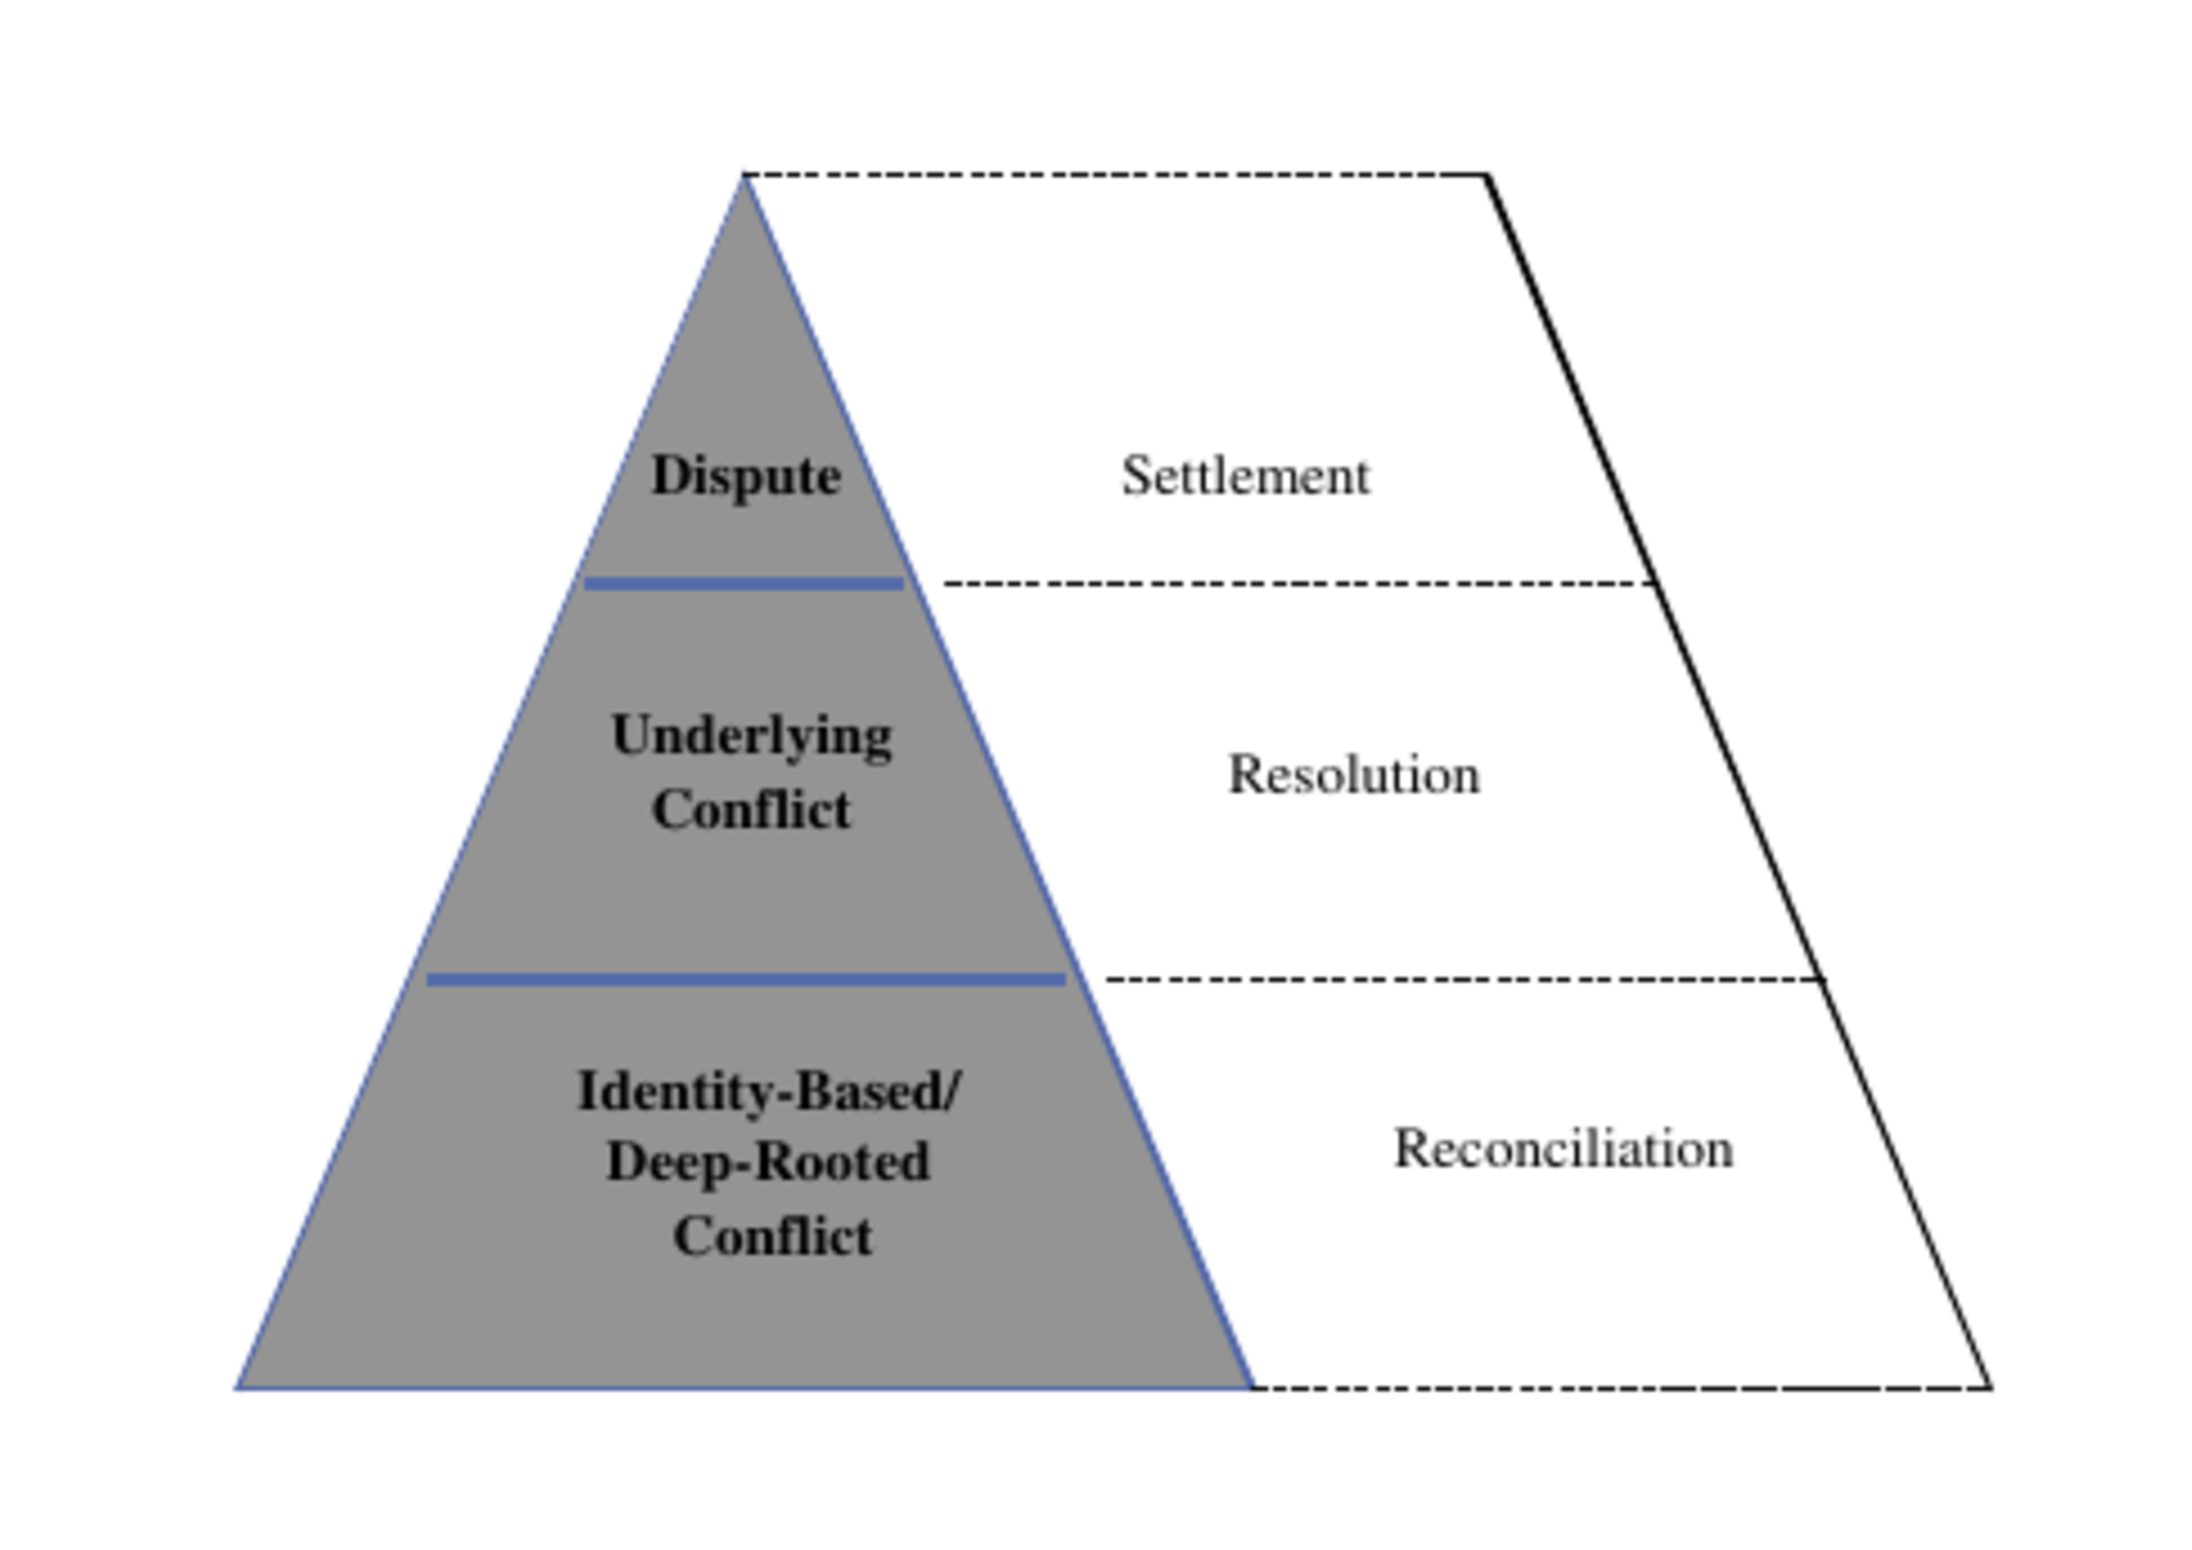
\includegraphics[width=0.8\textwidth]{/home/boer/doks/PhD/Tesis/Images/ConflictLevels}

\caption{\label{fig:The-conflict-triangle}The conflict triangle from \citet{Madden_n_McQuinn_2014}
showing different levels of conflict and the response needed to truly
\textquotedbl{}make peace\textquotedbl{}.}
\end{figure}


\paragraph{Process factors relate to decision-making design, equity and authority,
and how (and by whom) these are exercised (see also \citealp{Stone_et_al_2008}).
For example, just the size of Namibian farms makes any method that
depends on legal threat or compliance checking impractical, if it
is not supported by the farmer who owns and manages the land. Where
farmers feel excluded from the decision-making process about predators
that will ultimately influence their livelihoods, the situation often
deteriorates into one where farmers \textquotedbl{}shoot, shovel and
shut up\textquotedbl{} (\citealp{Hoogesteijn_n_Hoogesteijn_2010};
various Namibian farmers, personal communication). \citet{Montag_2003}
mentions that \textquotedbl{}much of the conflict is around the control
of landowner land, government intervention, and private land rights\textquotedbl{},
also hinted at by \citet{Rust_et_al_2016} and \citet{Rust_2016*}.
\citet{Madden_n_McQuinn_2014} mentions that conservationists and
governments often resist giving up decision-making control, because
they already have the law on their side or they may fear what will
happen when stakeholders who seem less committed, or even antagonistic
to conservation objectives, are given a legitimate voice in decision-making.
However, in practice, working together is much more likely to result
in win-win solutions (sustainable coexistence). It is thus interesting
that almost all compensation schemes that had some level of success,
were those in which the livestock owners participated actively in
the decision-making process \citep{Stander_et_al_1997c,Lukarevsky_2003,Mishra_et_al_2003}
and thus shared ownership of the final solutions. }

\paragraph{\citet{Rust_et_al_2016} make the point that farmer-predator conflict
in Namibia also has politico-social and personal relationship aspects,
so that something that appears to have little connection to human-wildlife
conflict, namely the labour relations between farmers and their workers,
can have an effect on farmer-predator conflict. Building relationships
through transparency and trust, is the second aspect of reconciliation
needed for conflict resolution mentioned by \citeauthor{Madden_n_McQuinn_2014}.
They show the importance of such relationship building by the example
of conservationists finding a solution to human-elephant conflict
through asking questions and consulting with a local community, resulting
in a decision to use various kinds of fences. However, when they later
tried to apply the same method in other communities without a similar
period of consultation and trust relationship building, those same
methods did not succeed, with community members failing to implement
or maintain chilly peppers and breaking down fences. }

\paragraph{The final and perhaps most obvious part of resolving deep-rooted
identity conflict, involves the actual substance of practical and
cost-effective methods to mitigate farmer-predator conflict. Here
the suitability of a certain method to conditions on a certain farm
has often not been considered sufficiently. A number of researchers
have mentioned that predation losses does not seem to be uniformly
distributed, even within the same district \citep{Conradie_n_Piesse_2013},
and some farmers might have extremely high depredation losses, while
the majority have relatively few losses \citep{Van_Niekerk_2010}.
This appears to be an international feature of farmer-predator conflict,
with similar reports for example, from Slovakia \citep{Rigg_et_al_2011}
and the USA \citep{Shelton_2004}. But different levels of depredation
also imply that different management decisions and different anti-predation
methods are required.}

\paragraph{To summarize some of the main reasons why past human-carnivore conflict
mitigation approaches still fail to reduce the conflict:}
\begin{enumerate}
\item They often approach the conflict from either an ecological, conservationist
viewpoint only or from an agricultural, short-term economic viewpoint
only. Conservationists therefore frequently advise farmers to use
eco-friendly methods that are impractical or not economically viable.
Agriculturalists, on the other hand, often advise methods that appear
to give short-term results, but are not sustainable in the long run
and might actually aggravate the situation.
\item They usually only directly address the human-predator conflict itself
and only recently started taking into account the social aspects of
human-human conflict. But even so, the focus is often on social aspects
of the conflict that might at best be a contributing factor (e.g.
\citealp{Rust_et_al_2016}) while ignoring the deeper levels of conflict
\citep{Madden_n_McQuinn_2014} between the ecological and the agricultural
basic starting points \citep{Nattrass_n_Conradie_2013} that might
be the most important reason why farmers are unwilling to risk or
trust in \textquotedbl{}new\textquotedbl{} methods. Farmers themselves
often feel left out and not well represented as partners in predator
management decisions and advice (e.g. \citealp{Bergman_et_al_2013}
when commenting on \citealp{Daly_et_al_2006}). The importance of
farmers as full partners in predator conservation on farmlands, and
the final implementers of any HWC mitigating methods, as well as having
to personally bear the brunt of all costs and risks, is seldom explicitly
recognized. Farmers associations and agricultural unions are seldom
put in the situation where they can share ownership of ecologically
sound solutions to human-wildlife conflict (\textit{cf} \citealp{Lukarevsky_2003}).
\item Past approaches very seldom (if ever) take cognisance of the differences
between individual farms and farmers with regards to both ecological
and agricultural aspects of the situation. The approach is often that
of \textquotedbl{}one size fits all\textquotedbl{}.
\item Conservationists in particular are often guilty of not spelling out
the known drawbacks and limitations of proposed solutions to livestock
depredation and HWC, thereby creating unrealistic expectations (see
for example \citealp{Smuts_2008,Daly_et_al_2006}). When farmers run
into these, often unexpected, issues, they can become discouraged
and return to their known and trusted (even if not very effective)
\textquotedbl{}traditional\textquotedbl{} and unsustainable management
practices. Not only do they personally abandon any of the possibly
more effective methods, but typically they also spread the word that
a certain method \textquotedbl{}did not work for me\textquotedbl{},
discouraging other farmers from attempting it as well \citep{Shivik_et_al_2003}.
Not only the ignorance of limitations, but also the incorrect implementation
of methods can end in failure, with the same negative end result.
\item \citet{Rust_2016*} found that the single most popular method for
mitigating HWC was conservation education and husbandry training to
reduce livestock depredation. It is often amazing how little farmers
know about the general behaviour of the predators found on their land.
Not only farmers, but even behavioural ecologists, still have great
gaps in our knowledge of predator behaviour outside protected areas
\citep{Balme_et_al_2014}. As farms have become larger in order to
remain economically viable and farming methods are often more extensive
than they used to be \citep{Nattrass_n_Conradie_2013}, farmers often
also know surprisingly little about the behaviour of their own livestock
(especially their anti-predator behaviour). This lack of knowledge
can result in basic mistakes being made (like dehorning of all cattle),
leading to unnecessary livestock losses. The lack of significant effect
by any other method except the numbers of wildlife on farms in Namibia
found by \citet{Marker_et_al_1996}, might be confirmation of the
need for knowledge, showing that how well protection measures are
implemented is possibly more important than which method is used.
\item While often making the mistake of offering a \textquotedbl{}one size
fits all\textquotedbl{} solution to farmers for their livestock depredation
problems, the opposite mistake is made as well when scientists simply
suggest a whole range of possible (usually non-lethal) methods for
farmers to use \citep{Shivik_2004,Daly_et_al_2006,Shivik_2006,Smuts_2008,Stone_et_al_2008,Chardonnet_et_al_2010},
without giving them any comparative guidance on the effectiveness,
costs and limitations of the different methods. This makes it just
as difficult, if not impossible, for a farmer to choose the most appropriate
method(s) for his particular farm and circumstances.
\item Because farming is inherently risky, farmers tend to be risk-averse
and to keep to what they know. The problem with this approach is that
circumstances have changed and keep on changing. Methods that were
affordable and effective in the past, are so no longer because of
changes in costs, legislation, ecological changes, etc.
\end{enumerate}

\section{How can we improve on past failures to resolve human-wildlife conflict?}

\paragraph{\citet{Shivik_2006} opined that future methods \textquotedbl{}need
to emerge from a mix of biology, sociology, and technology\textquotedbl{}.
It is well known that there is no silver bullet for human-wildlife
conflict \citep{Linnell_et_al_1996}. What works well against some
predators and in some circumstances, will fail in different situations.
And, except for permanently keeping all livestock in a barn and feeding
them, no method is 100\% effective in preventing livestock depredation
losses. The aim should be to find the most cost-effective and sustainable
method or combination of methods that fit the situation on a specific
farm. For this reason, \citet{Shivik_2004} proposed that livestock
depredation control should be approached similarly to Integrated Pest
Management (IPM). But it is not enough to know what method is most
likely to succeed, unless farmers are empowered to make the decision
for themselves using relevant knowledge, the uptake of better methods
for preventing farmer-predator conflict will probably remain low because
of the various social issues mentioned above. It is important that
the advantages, disadvantages and limitations of the various methods
available to a farmer should be known up-front before he commits himself
to implementing it on his farm. The process by which any specific
method is chosen and recommended should also be clear and transparent
to the farmer in order to avoid any unexpected nasty surprises during
implementation.}

\paragraph{So what should we do differently from what has already been tried?
It should be clear by now the the primary decision-maker and ultimate
implementer of any methods to decrease conflict with predators and
livestock losses, should be the livestock farmer himself, since he
will ultimately have to bear the costs of any method that he decide
on as well as having to deal with the consequences, whether good or
bad \citep{Yoder_2000}. It seems clear that conservation of larger
predators is not possible without including livestock farmers in the
process. But the common request for conservation education and husbandry
training \citep{Rust_2016*} show that farmers need the right information
in their hands on both the agricultural cost-effectiveness of different
methods and its ecological sustainability. One of the most important
aspects of applying any predation-prevention method, is the good record
keeping of the current situation on the farm \citep{Stone_et_al_2008}.
Knowing how much livestock is lost to predators, where most depredation
happens in the farm and which predators are responsible is basic knowledge
that is required in order to make good management decisions. \citet{Hoogesteijn_n_Hoogesteijn_2010}
actually consider it as a preventative method by itself. It should
be pointed out that good record-keeping is not necessarily correlated
to how intensive the farming system is. Even when livestock is only
seen once every six months, through the use of individual ear tags,
together with a weighing scale, the history of every cow can be recorded
and used in breeding and other management decisions. Computer expert
systems that capture expert human knowledge and use it in various
applications, have existed since the 1970s and became relatively popular
in the 1980s. A decision support system (DSS) is a specific type of
expert systems where the aim is not so much automation or artificial
intelligence, but to provide human decision makers with the relevant
information needed to make an informed decision \citep{Keen_1980,Sprague_1980}.}

\paragraph{Using a DSS avoids a number of the possible reasons for the past
failure of mitigating methods to reduce HWC. Because it is not a person
\textquotedbl{}telling the farmer what to do on his own farm\textquotedbl{},
at least part of the common underlying distrust of conservation scientists
\citep{Nattrass_n_Conradie_2013} or past bad experiences with specific
conservationists, is avoided (Axel Rothauge 2014, personal communication).
If the DSS is written in order to be transparent with regards to the
algorithms and data it uses, not only does it make it easier to trust
it, but if written as open source software, it can be updated and
improved as new knowledge and research becomes available. Ultimately
it would use feedback from farmers themselves who are using various
methods, to re-evaluate or update the basic data used (e.g. as costs
change or if more limitations of a specific method is found). A feedback
loop is thus built into the DSS allowing it to adapt to changing circumstances
(e.g. changes in costs of different methods). The algorithm used will
include both the short-term agricultural economic cost-effectiveness
of the various methods and the long-term ecological sustainability
in order to choose the most appropriate method for the specific situation
on a farm as entered by the farmer. This is in effect using an ecologically
holistic view of the farming system, looking at the whole ecosystem
and not considering livestock depredation as an isolated problem \citep{Bingham_1997}.
By presenting only the top three methods with their limitations, pros
and cons, the farmer will have the required information available
to make informed decisions on what to do to decrease livestock losses,
without being overwhelmed with irrelevant data. }

\section{Conclusions}

\paragraph{Many different approaches to human-wildlife conflict have been used
in the past, with partial success. Many farmers still prefer to kill
predators on their land or to engage in unsustainable farming practices,
without the issue being resolved. Human-wildlife conflict still remain
the major cause of death for many predators, but ultimately farmers
remain the custodians of predators on their land and need to be empowered
to do a better job of managing their land, including both agricultural
aspects and ecological aspects of farmer-predator conflict. An online
decision support system can put the relevant knowledge into the hands
of farmers who are struggling with livestock depredation on their
land. It can also be updated periodically, making sure that it remains
current. In time, the model can be expanded or adapted to include
communal farming systems \citep{Blackburn_et_al_2016} and other predators.}

\bibliographystyle{/home/boer/TeX/bibtex/bst/stellenbosch/myplainnat}
\bibliography{/home/boer/doks/PhD/Literature/Ecology}

%
\begin{comment}
\end{comment}


\chapter{A Probabilistic Graphical Model for Human-Wildife conflict}


\title{Building a Probablistic Graphical Model for Human-Wildife Conflict}

\author{Chavoux Luyt}
\maketitle
\begin{abstract}
Although many methods has been suggested to mitigate human-predator
conflict, it is still a worldwide and increasingly important problem,
both for predator conservation and for livestock farming. In the past
most solutions to this conflict has been either from an agricultural
perspective or from a conservation perspective. However, because the
goals of these two perspectives are seldom the same, there has been
frustratingly little progress in preventing human-wildlife conflict.
Here we review different published methods used worldwide to alleviate
human-wildlife conflict, specifically conflict between livestock farmers
and predators, the pros and cons of each method and the probable usefulness
of the different methods to livestock farmers in North Central Namibia.
We propose a more useful classification of methods than the usual
lethal non-lethal dichotomy, and compare the various methods in terms
of their success and cost-effectiveness. We also investigate the possible
reasons for both failures and successes of the different methods.
Lastly we propose that a new approach is needed if we want practical
and sustainable solutions to our current human-wildlife conflicts.
\end{abstract}

\section{Introduction}

\paragraph{Human-wildlife conflict is a growing global problem \citep{Messmer_2000,Treves_n_Karanth_2003b,Nyhus_et_al_2005}.
Land managers, specifically farmers, are key to finding sustainable
solutions to this conflict. One major reason why attempts at mitigating
farmer-predator conflict in the past have failed, is because the local
conditions on a specific farm has not been taken into account sufficiently.
And farmers did not always have the relevant information available
to decide on the best management strategy that will be both cost-effective
and sustainable in the long run. }

\paragraph{Farmlands are part of a wider ecosystem. Therefore both the ecological
sustainability and the agricultural cost-effectiveness of any proposed
solution, are critical to its success. Typically, ecological modelling
has fallen into two broad groups. Simulation models typically tries
to incorporate as many different parameters as possible and to be
as realistic as possible. Because of the huge number of parameters,
some of which might not be relevant, these kind of models often end
up as a \textquotedbl{}black box\textquotedbl{} with little guarantee
that it is actually true to the real situation and that all the relevant
factors have been included in the model. It is often no longer understandable
from a human perspective. The opposite approach is to simplify matters.
It is accepted that the model is not realistic representation of ecosystem.
Instead, the aim of the model is to gain a better understanding of
the ecosystem. It is a conditional model, basically saying that \textit{if
}certain conditions and assumptions are true \textit{then }certain
effects can be expected to result from it. It ignores all other influences
by concentrating only on those parts of the model that is relevant
to the specific question being asked. In the process, the model is
kept simple enough that it can be understood by humans.}

\paragraph{For livestock farmers to decide on the best solution for preventing
livestock depredation in their specific situation, it is important
that they are able to trust the output of a specific model. For this
reason, a model that is humanly understandable is more useful than
a possibly more realistic, but incomprehensible model. It is also
important that those agricultural aspects of the farming enterprise
that will play an important role in their decision, are included in
the model. Farmers are having to survive in uncertain circumstances
and explicit recognition of the uncertainty that is part of all farming,
can also help them to realize the limitations of management decisions
based on uncertain facts.}

\section{Why use Probabilistic Graphical Models (PGMs)?}

\paragraph{Our knowledge of farmland ecosystems are incomplete and thus necessarily
bound up with uncertainty. Historically there has been three approaches
to modelling uncertainty in computer systems:}
\begin{enumerate}
\item Fuzzy logic. Here statements are not considered as either true (1)
or false (0), but as having a certain degree of truth between 0 and
1, resulting in a multi-valued logic. This result in the counter-intuitive
result that f(A \ensuremath{\bigvee} \textlnot{} A) \ensuremath{\neq}
f(True). Whereas normally either a statement A or its negation NOT
A, would be true, this is not necessarily true in fuzzy logic. As
a result, although fuzzy logic based expert systems have been very
successful in commercial applications, these have tended to be rather
small, with limited levels of inference, and the various parameters
often need to be tuned using machine learning techniques. The fact
that it includes some obviously counter-intuitive statements, makes
it difficult to understand or explain and thus not really a good choice
for our use case. Additionally, farming systems and ecosystems are
complicated, making it difficult to model using fuzzy logic that are
better suited to smaller systems.
\item Dempster-Shafer modelling is another approach to dealing with uncertainty.
Instead of dealing directly with probabilities though, it deals with
the degree of evidence we have for certain truth values, called belief
functions. This can be a very useful approach in some circumstances.
However, the theoretical basis of this model and the situations for
which it is a good fit, are still debated. It is best used when there
are multiple independent sources of evidence with some overlap concerning
the same basic question (i.e. an accumulation of evidence). Because
it looks only at evidence, rather than at probabilities, it cannot
deal directly with cause and effect. It has been considered as a generalization
of probabilistic theory, and can be simpler to implement than the
Bayesian Network approach. However, it has no way to model cause and
effect naturally, and can only combine various pieces of evidence
for a certain outcome, without implying any causal relationship. One
possible advantage of this approach, is that an explicit value can
be assigned to uncertainty. However, it is easily misused for situations
where it is not a good fit and can give counter-intuitive or untrustworthy
results in such cases \citep{Josang_et_al_2010}.
\item Bayesian probability theory has a long history and is much better
understood than the previous two approaches from a mathematical point
of view. One important advantage compared to the other two types of
models, is that it provides a very natural method to model dependencies
and conditional dependencies, making it very intuitive to model real
cause and effect relationships between different factors. However,
it can be computationally expensive. Until recently, it was impossible
to model the joint probability distribution over any reasonable number
n of random variables taking x different values per variable. It would
require $x^{n}$ different probability assignments, which are both
computationally expensive and too large to fit into computer memory,
and incomprehensible to the human brain \citep{Koller_n_Friedman_2005}.
This remained the main barrier to using probabilistic methods for
solving problems dealing with uncertainty, until fairly recently when
the current methods of Probabilistic Graphical Models (PGMs) were
developed. The recent developments have resulted in PGMs based on
Bayesian probability theory becoming the dominant paradigm in most
modern expert systems in general and decision support systems in particular
\citep{Koller_n_Friedman_2005}. For these reasons, this approach
was chosen as the preferred one for modelling the different human-wildlife
mitigation methods.
\end{enumerate}

\paragraph{There are many different Probabilistic Graphical Models, but the
best fit for the kind of problem we are looking to solve for farmer-predator
conflict, would be a version of Bayesian Network (Koller 2016, personal
communication). A Bayesian Network is a Directed Acyclical Graph (DAG),
consisting of a number of nodes, representing random variables, connected
by directed edges, representing dependencies between the nodes and
a table with the conditional probability distribution for each node
given its parents. For the marginally independent nodes (those without
any parents) their probabilities are given by a prior probability
distribution. The basic Bayesian Network has been extended to a form
known as Influence Diagrams. In this type of model, not only the various
random variables and their conditional probability functions are described,
but additionally, there are }
\begin{enumerate}
\item action variable nodes, denoting actions that can be taken by humans
and 
\item utility nodes, denoting the expected utility that will result from
the chosen action.
\end{enumerate}

\paragraph{Running the model for each choice of anti-depredation method, a Maximum
Expected Utility (MEU) value can be calculated for that method. While
this MEU might not be an exact value denoting the true maximum expected
utility of each choice, it is robust for comparing the different methods,
since essentially the same model is used for each method and just
the parameters change, depending on the method. As in any other computer
program, the GIGO (garbage in, garbage out) principle still holds,
however. The results would still be dependent on the reliability of
the data provided by the farmer and the robustness of the assumptions
built into the model. Using a Probabilistic Graphical Model however,
the assumptions are stated explicitly as part of the model and can
be updated over time in order to improve the model.}

\section{The model - What data do we need to make an informed and useful decision?}

\paragraph{For livestock farmers to make an informed decision on the best anti-predation
method for their specific circumstances, both ecological and agricultural
information should be used. From a strictly (and short-term) agricultural
point of view, the cost and relative efficiency of the different methods
used to protect livestock from predation should be the most important
factor. Other agricultural aspects to be considered, include the available
infra-structure on the land, the availability of capital for farm
infrastructure improvements, the sustainable stocking rates of the
land, the long-term effects of the different techniques on the veld
quality, the kind and breeds of livestock (and the marketing and other
reasons for using these specific types), the topography and vegetation
types of the land, the density of available water points and the quality
and quantity of drinking water on the land, the size of the farm,
etc. }

\paragraph{However, especially for the long-term sustainability of whichever
method is used, a number of ecological aspects are important as well.
Two question concerning predator diet preferences can influence the
management of a livestock farmer: }
\begin{enumerate}
\item The diet preferences (if any) of the predator species on his farm
impacting livestock or game production (i.e. if he can stock the farm
with cheaper, but preferred prey species, his high-value game or livestock
animals are less likely to be preyed on by these predators) and 
\item the importance of individual prey preference of the predators on his
land (i.e. if there are only some individuals that are preferring
livestock as prey, removing them from his land might be a viable management
option). 
\end{enumerate}

\paragraph{The habitat preferences of predators can influence his management
options in two ways: }
\begin{enumerate}
\item If different predator species (that prey on different kinds of livestock
or age classes) prefer different habitat types, it may be possible
to keep vulnerable livestock away from those high-risk habitats on
his farm (provided there is enough low-risk alternative areas available)
and 
\item if the reason why certain predators prefer certain habitat types within
their wide-ranging home ranges can be established (e.g. for hunting,
or by females with higher prey requirements for having their cubs),
vulnerable livestock can be kept away from these habitats. 
\end{enumerate}

\paragraph{Lastly, the interactions between the predator species can also influence
management options. It has been claimed that caracals can deter jackals
from some areas \citep{DuToit_2013} and it is known that leopards
will kill and eat blackjacked jackals \citep{Bothma_n_Le_Riche_1994},
and that caracals and jackals will occasionally kill each other's
young. One of the major reasons for the increasing problems with jackals
and caracals could be meso-predator release \citep{Beinart_1998},
but the extend and importance of these interactions have not been
studied in enough detail to know if it could be a significant reason
for the reported increase in livestock depredation. If meso-predator
release plays a role in Namibian ecosystems, it becomes important
for farmers to maintain enough larger predators on their land to prevent
future livestock losses from too many meso-predators.}
\begin{description}
\item [{A}] conceptual Bayesian Network model:
\begin{figure}[h]
\textit{\caption{Conceptual PGM to determine success probability of farmer-predator
conflict resolution methods. Grey nodes indicate data we need from
the farmer, white nodes the pre-existing model. The final value is
a probability that a specific method will be successful for a specific
farmer.}
}
\begin{description}
\item [{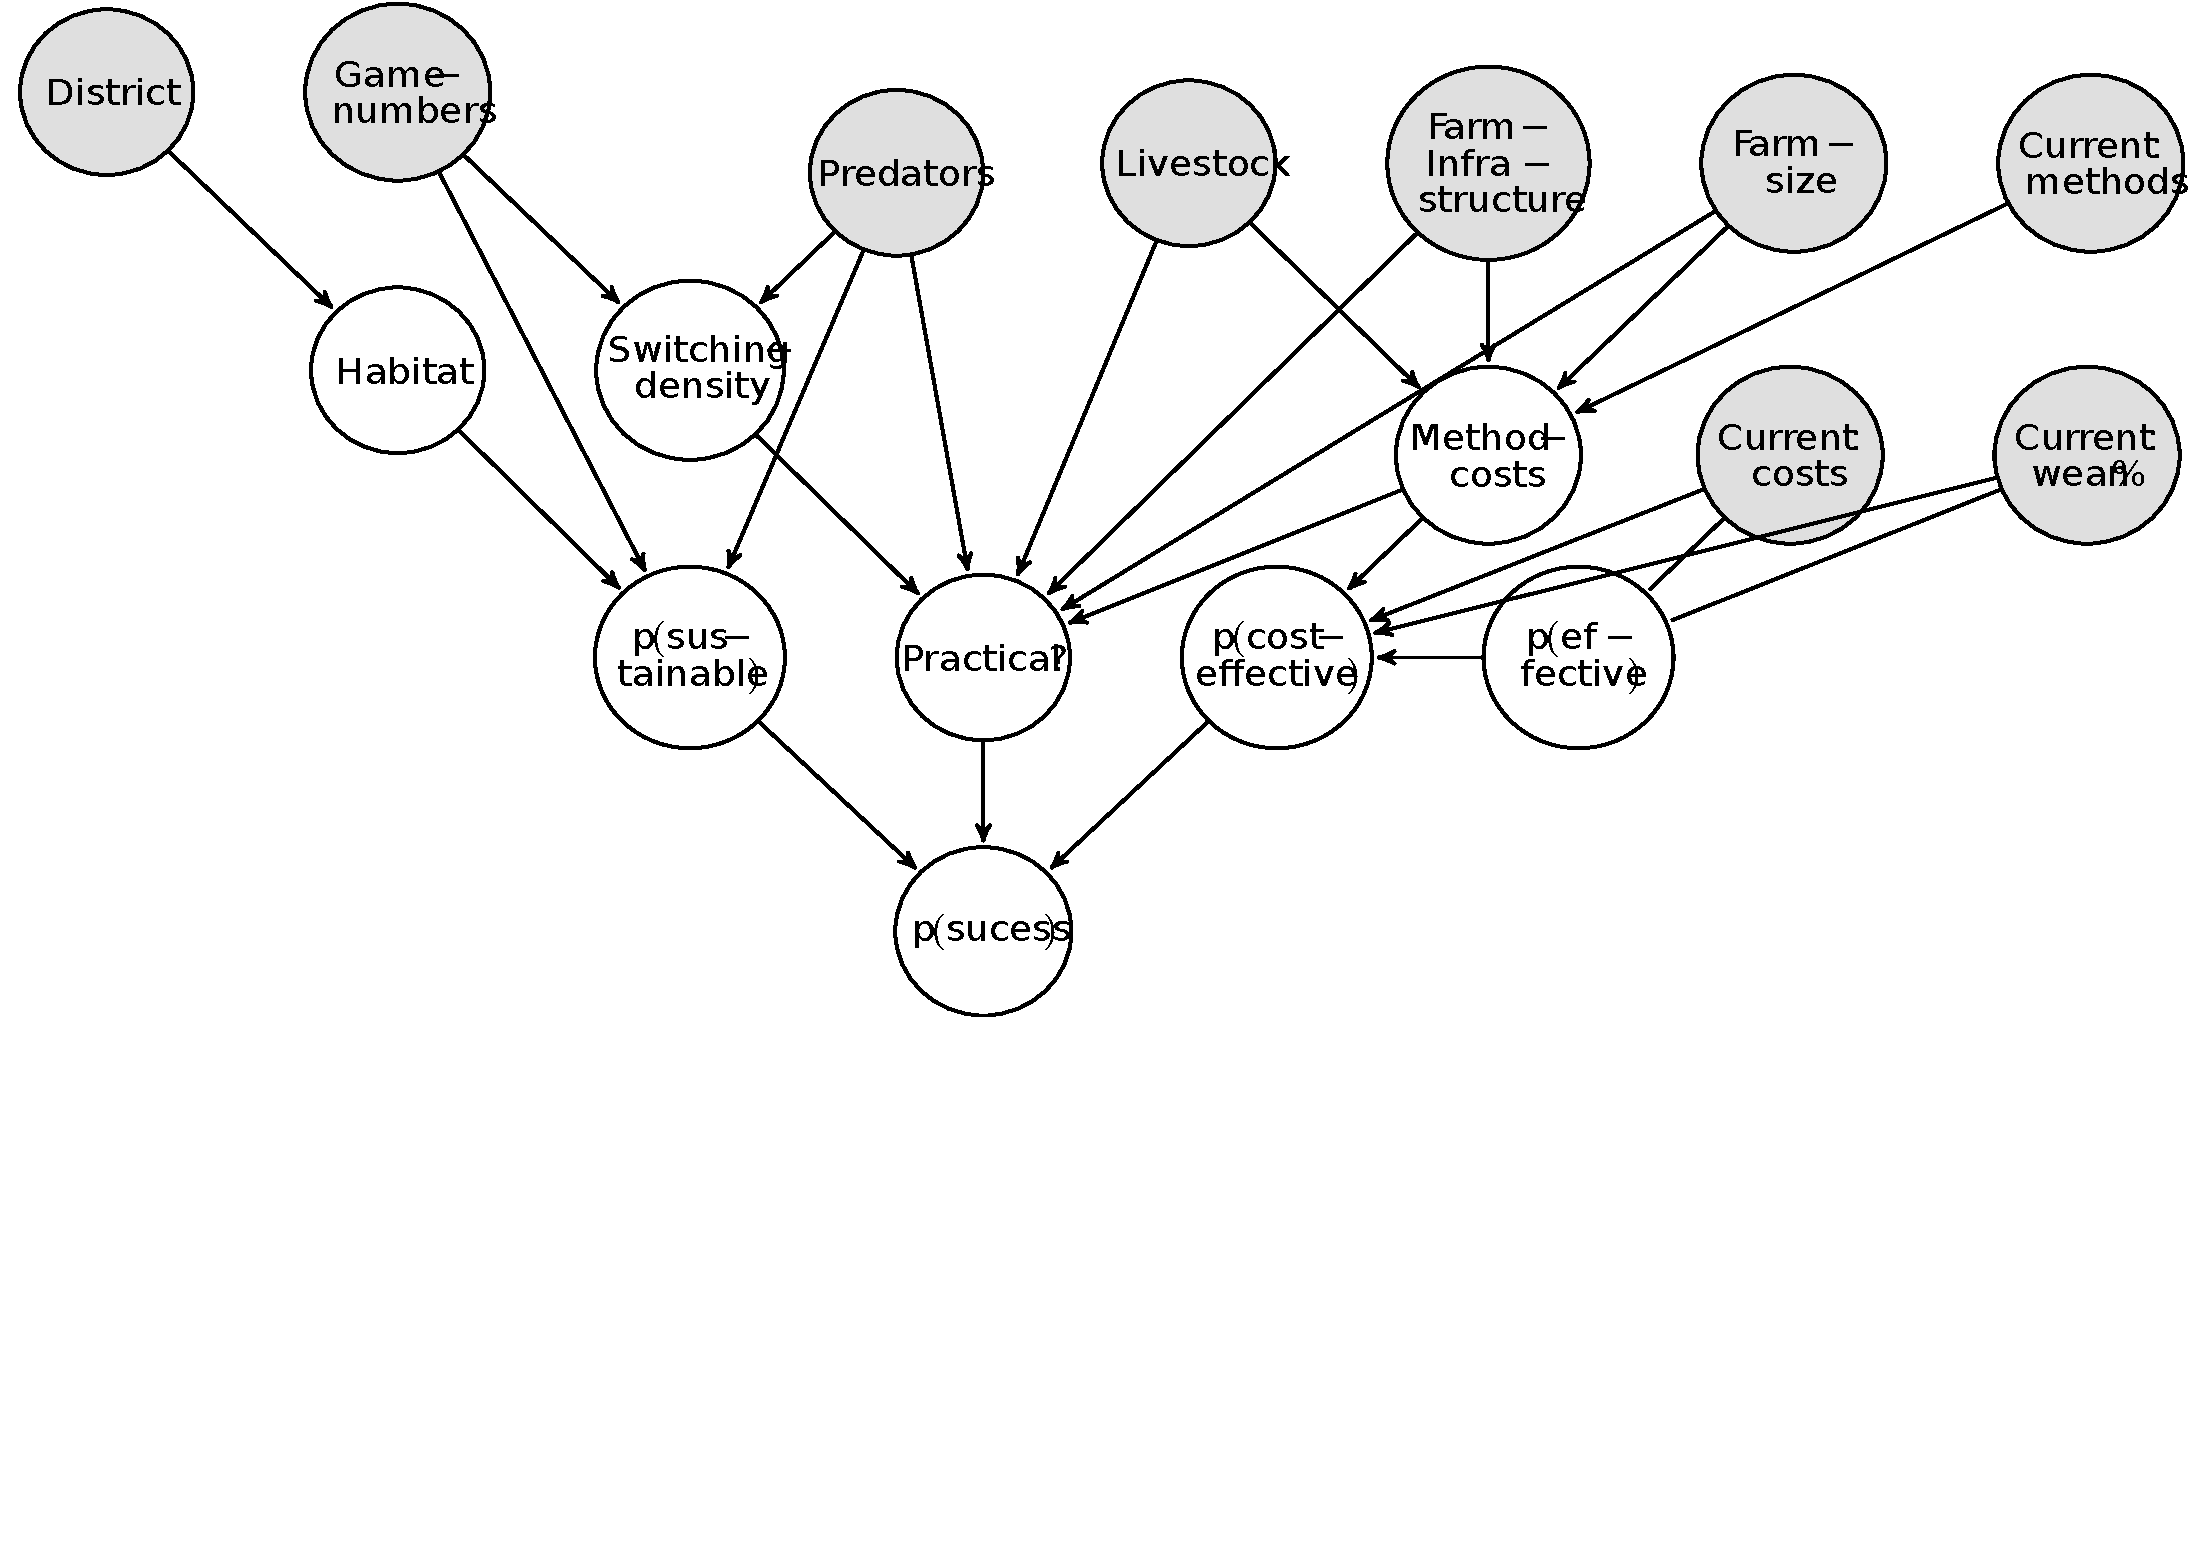
\includegraphics[width=0.8\paperwidth]{/home/boer/doks/PhD/Tesis/Images/FwP_Model}}]~
\end{description}
\end{figure}
\end{description}

\section{Constraints and limitations}
\begin{description}
\item [{What}] kind of data (which would be really useful) is unavailable
currently and in the foreseeable future? What are the uncertainties?
How can we work around these uncertainties to still get useful answers?
GIGO (Garbage in, garbage out): How do we prevent \textquotedbl{}garbage
data\textquotedbl{} from fouling our model? How can we adapt our model
to changing circumstances? How can we extrapolate the model to other
species and situations (e.g. more predator species, communal farmers,
other continents and biomes)?
\end{description}

\section{Refining our model}
\begin{description}
\item [{Using}] data from farmers using the online Decision Support System
to update our model automatically. Providing an easy way to update
our parameters as more research becomes available. Writing a transparent
model and keeping it simple enough to understand and update (the KISS
principle). Using alternative algorithms (e.g. Dempster-Shafer to
deal with uncertainty instead of pure Bayesian Networks). Open Source.
\end{description}

\section{Conclusions}

\paragraph{Many different approaches to human-wildlife conflict have been used
in the past, with partial success. Many farmers still prefer to kill
predators on their land or to engage in unsustainable farming practices,
without the issue being resolved. Human-wildlife conflict still remain
the major cause of death for many predators, but ultimately farmers
remain the custodians of predators on their land and need to be empowered
to do a better job of managing their land, including both agricultural
aspects and ecological aspects of farmer-predator conflict. An online
decision support system can put the relevant knowledge into the hands
of farmers who are struggling with livestock depredation on their
land. It can also be updated periodically, making sure that it remains
current. In time, the model can be expanded or adapted to include
communal farming systems \citep{Blackburn_et_al_2016} and other predators.}

\bibliographystyle{/home/boer/TeX/bibtex/bst/stellenbosch/myplainnat}
\bibliography{/home/boer/doks/PhD/Literature/Ecology}

%
\begin{comment}
\begin{description}
\item 
\end{description}
\end{comment}


\chapter{The Agricultural perspective: Farmer surveys}

\section{How big is the problem of livestock depredation and predator conflict
really in Namibia?}
\begin{description}
\item [{How}] widespread is Human-Wildlife Conflict involving farmers and
predators really in Namibia? Any geographical hotspots? How big are
farmers' losses? And what is happening to the predator populations
on farms (according to the farmers)?
\end{description}

\section{Baseline data to use for training the Probabilistic Graphical Model}
\begin{description}
\item [{Cost-benefit}] analysis of methods (+ other pros \& cons) currently
used by Namibian farmers (will be very rough at this stage, but the
best we have). Compared with South African data where available.
\end{description}

\chapter{Spatial behaviour and habitat preferences}

\section{Comparing the spatial behaviour of 4 predator species}
\begin{itemize}
\item Tracking: July 2014 - March 2015 - Good method \citep{Stander_et_al_1997b}
\item Literature for each species
\end{itemize}

\section{Spoor tracking: The good, the bad and the ugly}
\begin{description}
\item [{Use}] similar method to that for unmarked species to estimate (relative)
densities of predators and prey. Compare to camera trap estimates
(and game count data from farmer). Discuss advantages of spoor tracking
compared to other methods (Non-invasive, cheap, includes behavioural
data, continuous, etc.). Discuss disadvantages of spoor tracking (Good
trackers becoming scarce and few tracking schools to develop skills,
seldom able to ID individuals from tracks \textendash{} and thus bad
estimate of densities \textendash , possible skew to roads, the importance
of substrate and vegetation in tracking, some species more difficult
to track than others, etc.). 
\end{description}

\section{How to improve tracking as a tool for science.}
\begin{description}
\item [{FIT}] (Footprint Identification Technology) being developed, my
CyberTracker track app, citizen science, creating tracking jobs and
training schools, using in combination with other methods (dogs, drones
and/or camera traps).
\end{description}

\section{How the spatial behaviour of the 4 predator species feeds into our
PGM}
\begin{description}
\item [{The}] role of density, habitat preferences, intra- and inter-specific
avoidance, aggression and competition. Alternative sources for the
necessary data, seeing as how spoor tracking largely failed.
\end{description}

\chapter{Estimating predator densities from camera traps using Spatially Explicit
Capture-Recapture models. }

\section{Introduction}
\begin{itemize}
\item March - June 2014
\item Which predator species in area?
\item How many individual predators? Density estimates.
\item Leopard-Cheetah fluctuation: Perception (from surveys?), Reality (Cam.
trap data) and possible causes (Behavioural models).
\item Historical data: What do we have? How many individuals? What areas?
How long per individual? Data point frequency? What species? Did the
tagging periods (and place) overlap with the previous camera trap
surveys? What data has already been published and what can still be
used? (Relative Abundance Index)
\end{itemize}

\section{SECR for spotted cats}
\begin{description}
\item [{Determine}] cheetah and leopard densities using SECR and compare
with other studies in Northern Namibia.
\end{description}

\section{Determining densities for unmarked species}
\begin{description}
\item [{Try}] to determine jackal and caracal densities from the Camera
Trap studies using approximations when individuals cannot be identified.
Compare with published studies (for caracals in Namibia and outside
Namibia for jackals in comparable habitat). Use the same method to
estimate prey availability and density.
\end{description}

\section{Predator density and prey requirements}
\begin{description}
\item [{How}] predator density and prey requirements (including prey switching
to livestock at low wild prey densities - see \citet{Khorozyan_et_al_2015})
influence the model (PGM) for our DSS (Decision Support System)
\end{description}
\begin{comment}
For Testing how to include separate chapters:...\include{CamTrap}
\end{comment}


\chapter{The final Decision Support System (DSS)}

\section{User Interface of the DSS (Web application)}
\begin{description}
\item [{The}] DSS user interface will be a web application written in Python.
It consists of 3 parts: Specific inputs from the farmer, stored data
inputs (the model) and the outputs (see Figure \vref{fig:DSS}). 
\begin{figure}

\caption{\label{fig:DSS}\textit{The Decision Support System}}

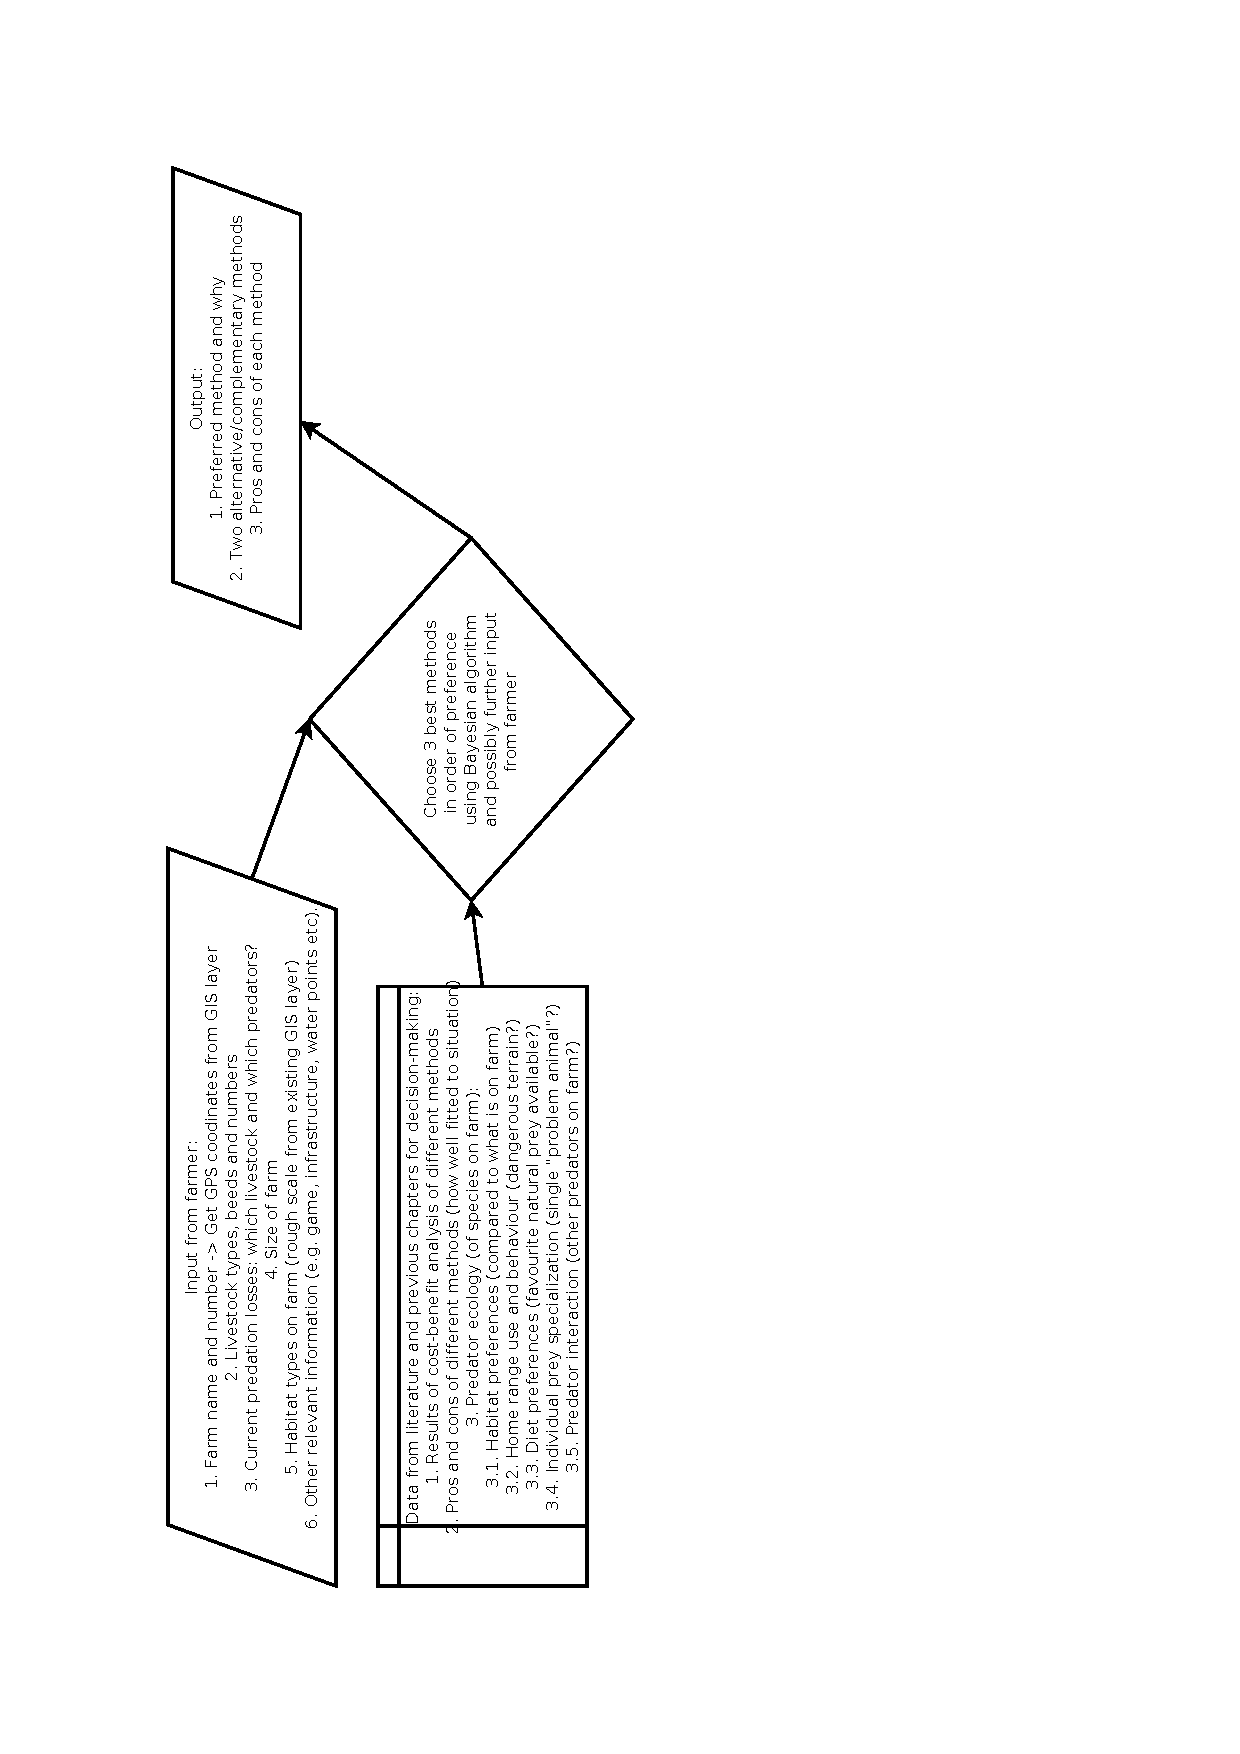
\includegraphics[angle=270,origin=ct,width=0.8\paperwidth]{Images/DSS1}
\end{figure}
\end{description}
\begin{itemize}
\item Inputs by farmers:
\begin{itemize}
\item Online interface, similar to survey from chapter 4.
\end{itemize}
\item Model (cf. chapter 3):
\begin{itemize}
\item Three parts with some overlap:
\begin{itemize}
\item Sustainability: Use biodiversity and stocking rates (compared to district
rainfall/vegetation type) as proxies for sustainability (maybe include
little human disturbance also).
\item Practical: Some methods can be excluded simply because they are impractical
in some situations; they are not simply too expensive or not effective;
they cannot be implemented at all for various reasons (e.g. a stud
farm cannot suddenly switch to another breed, or dogs with cattle,
or electrifying fences around large (20 000 ha +), mountainous farms,
or labour-intensive methods for part-time \textquotedbl{}weekend\textquotedbl{}
farmers).
\item Cost-effectiveness: How many weaners/female survive using the method/cost
spent implementing (also include costs of changing current methods
to start implementing it).
\end{itemize}
\item Include other methods from outside Namibia (identified in lit. review)
for discussion of pros and cons
\item Commercial vs communal: The results might not be applicable in most
of Africa? Communal excluded for now?
\item (How predators use their territories. Determining factors (Dempster-Shafer
model?).) Not practical for now?
\item Easy-to-use interface for non-programmers to change the model and
update data with new research
\end{itemize}
\item Outputs:
\begin{itemize}
\item Decision support system for farmers. With 3 top options and advantages
and disadvantages of each.
\item Extrapolate: Where are predators most likely to be? Does that correlate
to conservancies/communal land etc. ???
\end{itemize}
\end{itemize}

\section{Technology used in the DSS}
\begin{description}
\item [{Short}] discussion of the technology that was used for creating
the DSS, advantages and disadvantages, and lessons learned.
\end{description}

\section{Automatic update of DSS model}
\begin{description}
\item [{Using}] the input data from the farmers about their current methods,
to update the model over time. How garbage data is to identified and
filtered out. Also the possible use of data from CyberTracker App
to update the model.
\item [{Possibly}] include \textquotedbl{}feedback page\textquotedbl{}
where farmers can explicitly share their experiences.
\end{description}

\end{document}
